\chapter{Accessibility to oncology care}

\section{Context}

\subsection{Motivation}

While a lot of the ongoing research is focusing on finding new cancer treatments, accessibility to oncology care receives less attention. Yet, several studies have showed that access to health services plays a key role in cancer survival. For instance, geographic residency status and social environment seem to explain treatment and prognosis disparities for patients with non-small cell lung cancer \cite{johnson_treatment_2014}. In France, increases in travel times to health services were associated with lower survival rates for patients with a colorectal cancer \cite{dejardin_influence_2014}. In New Zealand, living in deprived areas, far from a cancer center or from primary care was associated with lower survival chances for patients with colorectal, lung and prostate cancers \cite{haynes_cancer_2008}.

\subsection{Accessibility definition}

Accessibility refers to the relative ease by which services can be reached from a given location \cite{wang_measurement_2012}. Accessibility can be defined by spatial factors, determined by where you are; and non-spatial factors, determined by who you are \cite{khan_integrated_1992}. \ac{sa} methods assess the availability of supply locations from demand locations, connected by a travel impedance metric. Supply locations are characterized by their capacity or quantity of available resource. Similarly, demand locations are characterized by their population. Such methods have been successfully used to measure access to healthcare, such as primary care \cite{guagliardo_spatial_2004} or oncology care \cite{wang_measurement_2012,zahnd_spatial_2021,alahmadi_spatial_2013} in several countries including France \cite{launay_methodology_2019,gusmano_disparities_2014,gao_assessment_2016}. In what follows, we restrict accessibility to \acf{sa} and use both terms interchangeably.

\subsection{\acf{sa} methods}

There are several ways to compute accessibility to healthcare as reviewed in \cite{guagliardo_spatial_2004}. We detail these methods in the following sections.

\subsubsection*{Provider-to-population ratios}

% Definition
The easiest and most straightforward \ac{sa} method is to compute provider-to-population ratios, also referred as supply ratios. The ratio involves some indicator of health service capacity (supply) as numerator; while the denominator is the population size within the area (demand). For instance, when measuring accessibility to primary care, one might use the number of physicians in the area as supply, and area population as demand. The resulting ratio might be interpreted as the number of physicians per 100,000 inhabitants \cite{schonfeld_numbers_1972}.

% Pros
Supply ratios are highly interpretable, and relevant for comparisons of supply in large areas. Policy analysts have used these metrics to set minimal standards of supply and identify under-served areas where supply should be increased  \cite{schonfeld_numbers_1972,council_on_graduate_medical_education_physician_1998,connor_competition_1995}

% Cons
However, supply ratios have limitations that often prevent their usage in more detailed analysis. First, they do not account for patient border crossing, which commonly occurs for small areas \cite{connor_measuring_1994,basu_border-crossing_1996,basu_medicare_1995,holahan_border_1993}. Second, supply ratios are constant within the bordered area, which will lead to imprecision and false generalization in large areas. Finally, they do not consider travel impedance, which plays a major role in \ac{sa}. Consequently the results and interpretations can vary greatly depending on the size, number and configuration of the areal units studied. This problem is well-known to geographers and spatial analysts as the modifiable areal unit problem (MAUP) \cite{openshaw_modifiable_1983}.

\subsubsection*{Travel impedance to providers}

% Definition
As stated earlier, travel impedance is a key aspect of \ac{sa} evaluation. It is typically measured from a patient's residence or from the centroid of a population location when the precise location is not available. The impedance can be expressed in different ways: euclidean (straight) distance, travel distance or estimated travel time.

% Pros
Travel impedance is suited for rural areas, where providers are limited and patients often travel to the nearest choice available.

% Cons
However, travel impedance is less relevant for urban areas. Indeed, there are numerous reasonable options available at a similar distance and patients won't travel to the closest one anymore. Moreover, travel impedance is a poor indicator of availability and should be combined with supply to properly evaluate \ac{sa} \cite{fryer_multi-method_1999}.

\subsubsection*{Gravity models}

% Definition
Gravity models are more sophisticated ways to evaluate \ac{sa}, based on a modified version of Newton's Law of Gravitation. They were initially developed to predict retail travel \cite{reilly_law_1931} and help with land use planning \cite{hansen_how_1959}. Gravity models combine both accessibility and availability, and work well in urban and rural settings. Gravity models represent the influence of all service points located within a reasonable distance from a population location. The influence is discounted by the increasing distance or travel impedance. The simplest formula for gravity-based accessibility is:

\begin{equation}
    A_i = \sum_j \frac{S_j}{d_{ij}^{\beta}}
\end{equation}

In this equation, $A_i$ is the accessibility score at population location $i$. $S_j$ is the capacity of the service point $j$, and $d_{ij}$ the travel impedance (e.g. distance or travel time) between population location $i$ and service point $j$. We set $\beta$ as a gravity decay coefficient, sometimes referred to as the travel friction coefficient. Intuitively, $\beta$ represents the change in difficulty of travel as the impedance value increases. The accessibility score increases with higher provider capacity, and decreases with higher travel impedance. Gravity models are an elegant way to compute accessibility, which accounts for border crossing, local variations, and travel impedance.

% Cons
The main drawbacks of this approach is the lack of intuitiveness, and healthcare policy makers prefer to think of \ac{sa} in terms of provider-to-population ratios or simple distance. Second, it only models supply and does not account for demand. Providers should not be equally accessible if they serve population locations with drastically different population sizes.
A proposed solution is to add a population demand factor $V_j$, to the denominator \cite{joseph_measuring_1982}:

\begin{equation}
    V_j = \sum_k \frac{P_k}{d_{kj}^{\beta}}
\end{equation}

Here, $P_k$ is the population size at population location $k$, and $d_{kj}$ is the distance between the population location $k$ and provider location $j$. Intuitively, the demand on provider location $j$ is obtained by summing the gravity discounted influence of all population points within a reasonable distance. The improved gravity model is:

\begin{equation}
    A_i = \sum_j \frac{S_j}{d_{ij}^{\beta} V_j}
\end{equation}

However, another problem is that the distance decay coefficient, $\beta$, is usually unknown and hard to estimate. Its form and magnitude can vary greatly with the service type and population under study \cite{talen_assessing_1998}.

\subsubsection*{\acf{2sfca}}

Recently, a new type of method has been developed and is now used in most \ac{sa} papers. This algorithm is called \ac{2sfca} \cite{luo_using_2004}. It is a two-step method that first computes a provider-to-population ratio for each provider location. In the second step, for each population location, an accessibility score is obtained by summing the provider-to-population ratios. For the algorithm to work, a catchment threshold (distance or travel time) must be set. Above this threshold, a provider location is considered unreachable from the population location, and vice versa.

\subsubsection*{\acf{e2sfca}}

The \ac{2sfca} method does not account for distance decay: a provider is either reachable or not. The \ac{e2sfca} \cite{luo_enhanced_2009} addresses this limitation by applying weights to differentiate travel zones in both steps.

Consider $P_i$ the population at location $i$, with $1 \leq i \leq n$ where $n$ is the number of population locations. Similarly, consider $S_u$ the capacity of care center $u$, with $1 \leq u \leq m$ where $m$ is the number of care centers. Finally, let $d_{iu}$ be the matrix of size $n \times m$ containing the distances between location $i$ and providers $u$. We consider $r$ sub-catchment zones each associated with a weight $W_s$, and a distance $D_s$, with $1 \leq s \leq r$, such that $D_1 < D_2 < ... < D_r$ and $W_1 > W_2 > ... > W_r$. The resulting r travel intervals are $I_1=[0, D_1], I_2=[D_1, D_2 ], ... ,I_r=[D_{r-1}-,D_r]$. The accessibility $A_i$ of a population location $i$ is computed in two steps:

\begin{itemize}
    \item Step 1: for every care center $u$, compute its weighted capacity-to-population ratio $R_u$.
    \item Step 2: for every population location, compute $A_i$ as the sum all the weighted $R_u$ of the reachable providers.
\end{itemize}

\begin{align}
    R_u &=  \frac{S_u}{\sum_{s=1}^{r} W_s \sum_{i, d_{iu} \in I_s} P_i} \\
    A_i &= \sum_{s=1}^{r} W_s \sum_{u, d_{iu} \in I_s} R_u
\end{align}

\subsubsection*{Multi modal \acl{2sfca}}

The \ac{e2sfca} methodology can be enhanced by incorporating both public and private transport modes \cite{langford_multi-modal_2016}. The proposed model yields separate accessibility scores for each modal group at each demand point to better reflect the differential accessibility levels experienced by each cohort.

Suppose that each method of travel (car, bus, walking, etc.) necessitates a dedicated transport network and let each such network be referred to as $N_1, N_2, ..., N_M$. In order to accommodate independent networks for each travel mode into the \ac{e2sfca} model, the computation of Step 1 becomes:

\begin{equation}
    R_u =  \frac{S_u}{\sum_{m=1}^{M} \sum_{s=1}^{r} W_{s,m} \sum_{i, d_{iu,m} \in I_s} P_{i,m}} \\
\end{equation}

Similarly for Step 2:

\begin{equation}
    A_i = \sum_{m=1}^{M} \sum_{s=1}^{r} W_{s, m} \sum_{u, d_{iu} \in I_s} R_u
\end{equation}

\subsubsection*{Huff model and \acl{2sfca}}

The \ac{e2sfca} does not consider competition among multiple healthcare sites available for a population location \cite{wan_three-step_2012}, and therefore it may lead to overestimation for some sites \cite{luo_integrating_2014}. The Huff Model is a widely accepted method for quantifying the probability of people's selection on a service site out of multiple available ones \cite{huff_probabilistic_1963}. It specifically aims to estimate/model people's choice on a service site with two factors: (1) distance to the service site; and (2) the attraction of the service site.

\begin{equation}
    Prob_{i,j} = \frac{C_i d_{ij}^{-\beta}}{\sum_{s \in D_0} C_s d_{is}^{-\beta}}
\end{equation}

Where:

\begin{itemize}
    \item $Prob_{i,j}$ is the probability of population location $i$ visiting service site $j$
    \item $d_{ij}$ is the travel time between $i$ and $j$
    \item $\beta$ is the distance impedance coefficient
    \item $C_j$ is the capacity \/ attractiveness of service site $j$
    \item $s$ is any service site within the catchment $D_0$ of $i$
\end{itemize}

Incorporating into the \ac{e2sfca} steps gives:

\begin{align}
    R_u &=  \frac{S_u}{\sum_{s=1}^{r} W_s \sum_{i, d_{iu} \in I_s} Prob_{i,u} P_i} \\
    A_i &= \sum_{s=1}^{r} W_s \sum_{u, d_{iu} \in I_s} Prob_{i,u} R_u
\end{align}

\section{Methods}

We computed the \ac{sa} score to these care centers for every municipality in metropolitan France, using the \ac{e2sfca} algorithm and oncology activity as supply variable. We compared the accessibility distributions with \ac{e2sfca} vs. regular \ac{2sfca}. The accessibility was lower with \ac{e2sfca} because of the weight decay. We also studied the influence of the supply variable in the accessibility score. Accessibility is much higher if we use the number of \ac{mco} stays as supply, instead of the oncology activity. This makes sense since oncology care centers are less common and the overall \ac{mco} activity is higher than the oncology activity.

\section{Results}

The oncology accessibility is unevenly distributed across the country, as displayed on \cref{fig:accessibility-france}. For better readability, we cut the accessibility scores into 5 quantiles. Q5 colored in dark green contains the top 20\% accessibility municipalities, and Q1 in light yellow contains the bottom 20\% ones. The lowest accessibility zones are mostly located in the center of the country and in mountainous regions like the Alps or the Pyrenees. Plot (B) shows that most of the population (51.6\%) lives in top 20\% accessibility municipalities, while 6.3\% lives in the bottom 20\% quantile. On map (A), care centers are displayed as squares, colored by cluster index, and sized by oncology activity. We see that accessibility is highest near the most specialized care centers. Indeed, the proportion of care centers from specialized clusters decreases in lower accessibility quantiles (C). We then ranked the departments by median accessibility and showed the top-10 and bottom 10 on plot (D). Among the top-5 departments, 4 are in Ile-de-France. Departments from the bottom-10 are rural or mountainous areas like Lozère and Alpes-de-Haute-Provence.  We notice disparities within departments as well, as outlined by the large interquartile range in Hérault or Alpes-Maritimes. On the contrary, this spread is very narrow in Ile-de-France departments.

\begin{figure}[H]
    \includegraphics[width=0.9\textwidth]{images/camion/fig2_accessibility_france.png}
    \centering
    \caption{
        \textbf{Distribution of the accessibility score computed with the \ac{e2sfca}, in metropolitan France.} Plot (A) shows municipalities colored by accessibility quantile. The care centers are drawn as squares, colored by cluster, and sized by oncology activity. Plot (B) shows the total population by accessibility quantile. Plot (C) displays the percentage of care centers by cluster by accessibility quantile. Plot (D) shows the top 10 and bottom 10 list of the departments, ranked by median accessibility.
    }
    \label{fig:accessibility-france}
\end{figure}

Accessibility score should be put into perspective with population density. Overall, the denser municipalities have a median accessibility around 0.02. Municipalities with low population densities have more extreme values.  \cref{fig:accessibility-vs-density} compares accessibility and population density for three different regions: Provence-Alpes-Cote-d'Azur (A), Ile-de-France (B), and Bourgogne-Franche-Comté (C). Municipalities are displayed as squares, colored by accessibility quantile, and sized by population density. These regions show very different profiles. In Provence-Alpes-Cote-d'Azur (A), accessibility is essentially low in non-dense municipalities near the Alps. However, in Bourgogne-Franche-Comté (C), we see dense municipalities with poor accessibility scores, representing a large proportion of the region. We also drew similar maps (D, E and F) where municipalities are colored based on the average travel duration for patients with cancer in 2018. We see that the average travel time is higher in municipalities with poor accessibility scores.

\begin{figure}[H]
    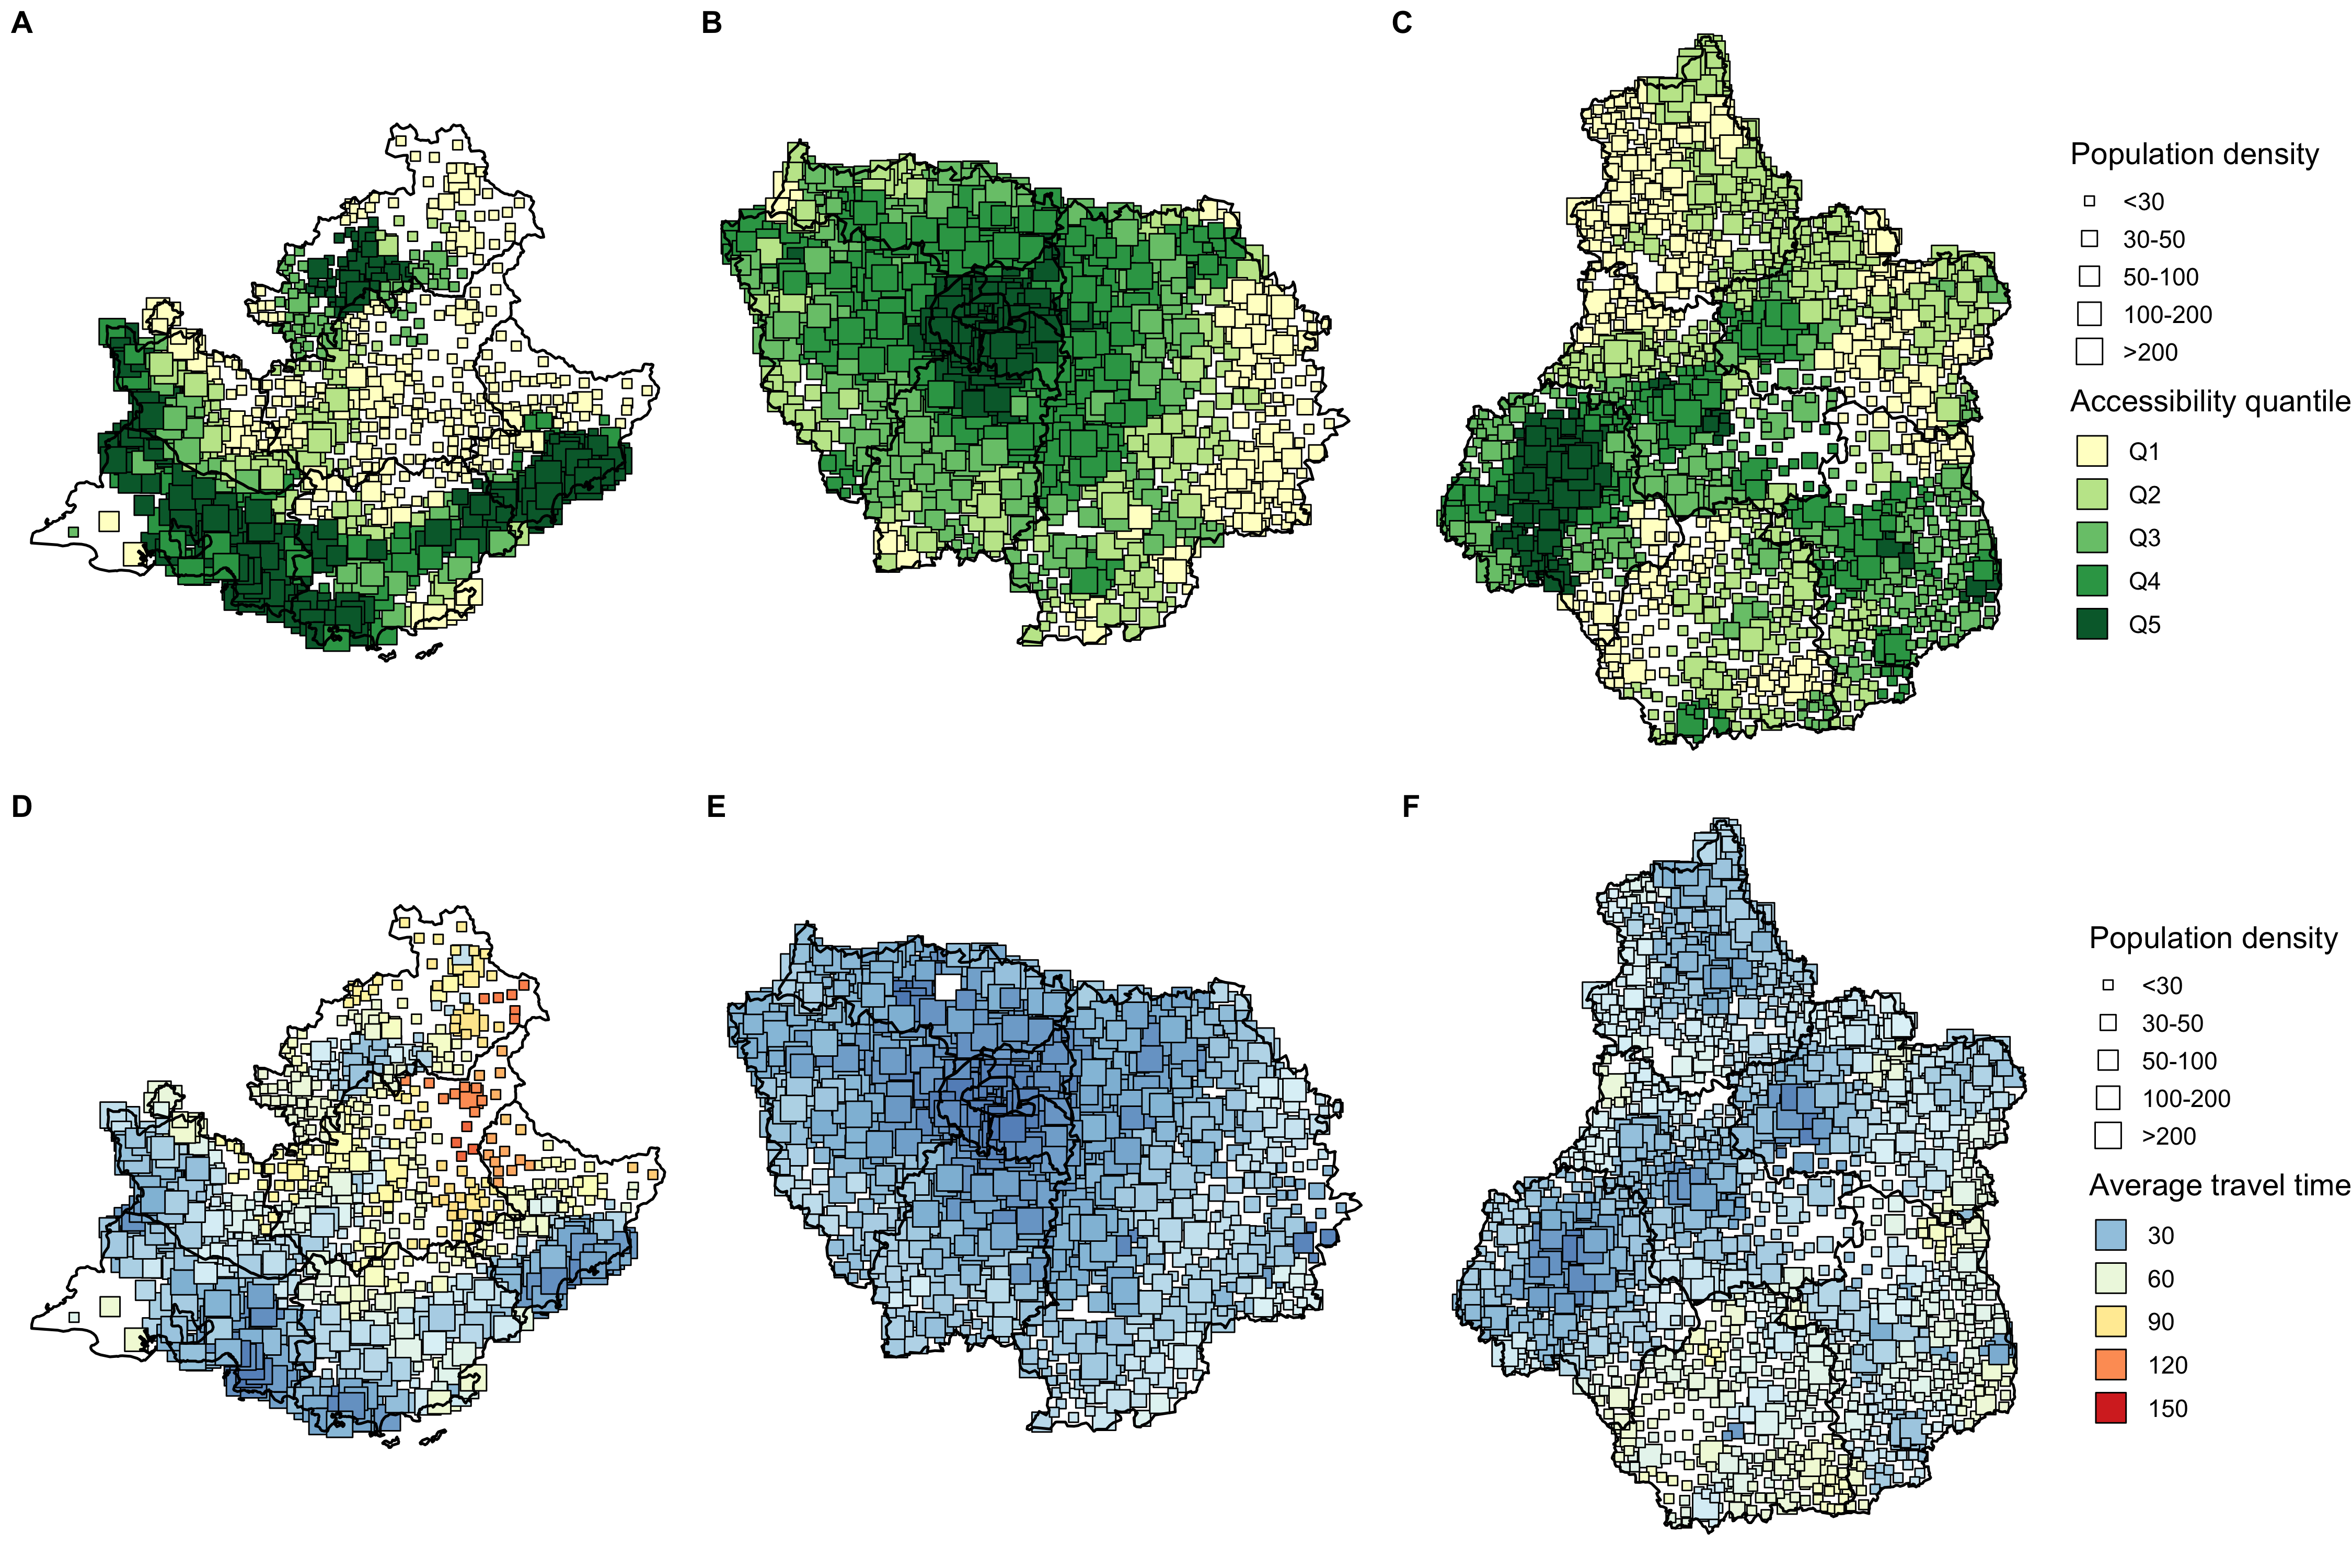
\includegraphics[width=0.9\textwidth]{images/camion/fig3_accessibility_vs_density_scatter_map.png}
    \centering
    \caption{
        \textbf{Comparison of population density with accessibility scores and patient average travel time for cancer pathways.} Showing results in three regions: Provence-Alpes-Cote-d'Azur (A, D), Ile-de-France (B, E) and Bourgogne-Franche-Comté (C, F). Municipalities are drawn as squares, sized by population density and colored by either accessibility quantile (A, B, C) or patient average travel time (D, E, F).
    }
    \label{fig:accessibility-vs-density}
\end{figure}

Finally, we compared our accessibility score with the department exit ratio, by municipality. Department exit ratio is defined as the proportion of cancer patients who visited a care center outside from their department of residence and was computed using the \ac{pmsi} database. In Provence-Alpes-Cote-d'Azur, the exit ratio is higher in departments with low accessibility scores and few oncology specialized care centers, as in Alpes-de-Haute-Provence and Hautes-Alpes. While the Var department has some oncology centers, exit ratio remains high since larger care centers are in Marseille and Nice.

\subsection*{Provence-Alpes-Cote-d'Azur}

We now focus on the region Provence-Alpes-Cote-d'Azur. This region is the far southeastern on the mainland. The region's population was 5,048 million in 2018. Its prefecture and largest city is Marseille. The region contains six departments. Bouches-du-Rhone, Var and Alpes-Maritimes are located on the coastline and gather the largest cities like Marseille, Nice, or Toulon. Alpes-de-Haute-Provence, Vaucluse, and Hautes-Alpes are inland departments, with a majority of rural and mountainous areas. Results are shown on \cref{fig:accessibility-paca}. By comparing maps (A) and (B), we confirm that the accessibility is maximum in denser areas of the region. Average patients travel time are displayed on map (C) and we drew the major roads (primary, motorway and truck) in red. The road system is well developed on the coast, rallying the larger cities of the region. However, driving from the rural areas in the Alps to the major cities is hard, resulting in higher travel times. The accessibility is unevenly spread within the departments, especially in Alpes-Maritimes where the distribution is multi-modal (D). There, cities like Nice and Cannes have large hospitals thus good accessibility, while the northern areas of the department are mostly mountains. Accessibility is higher in municipalities with dense populations, for all the departments (E). Finally, the average travel time decreases when the accessibility score increases. This makes sense since the accessibility score was computed based on the driving distance between population locations and care centers. However, it confirms that patients living in poor accessibility zones effectively travel further to seek oncology care. In Bouches-du-Rhone, nearly all the municipalities have an average travel time lower than 30 minutes, while in Alpes-de-Haute-Provence, average travel times are rarely lower than 60 minutes (F).

\begin{figure}[H]
    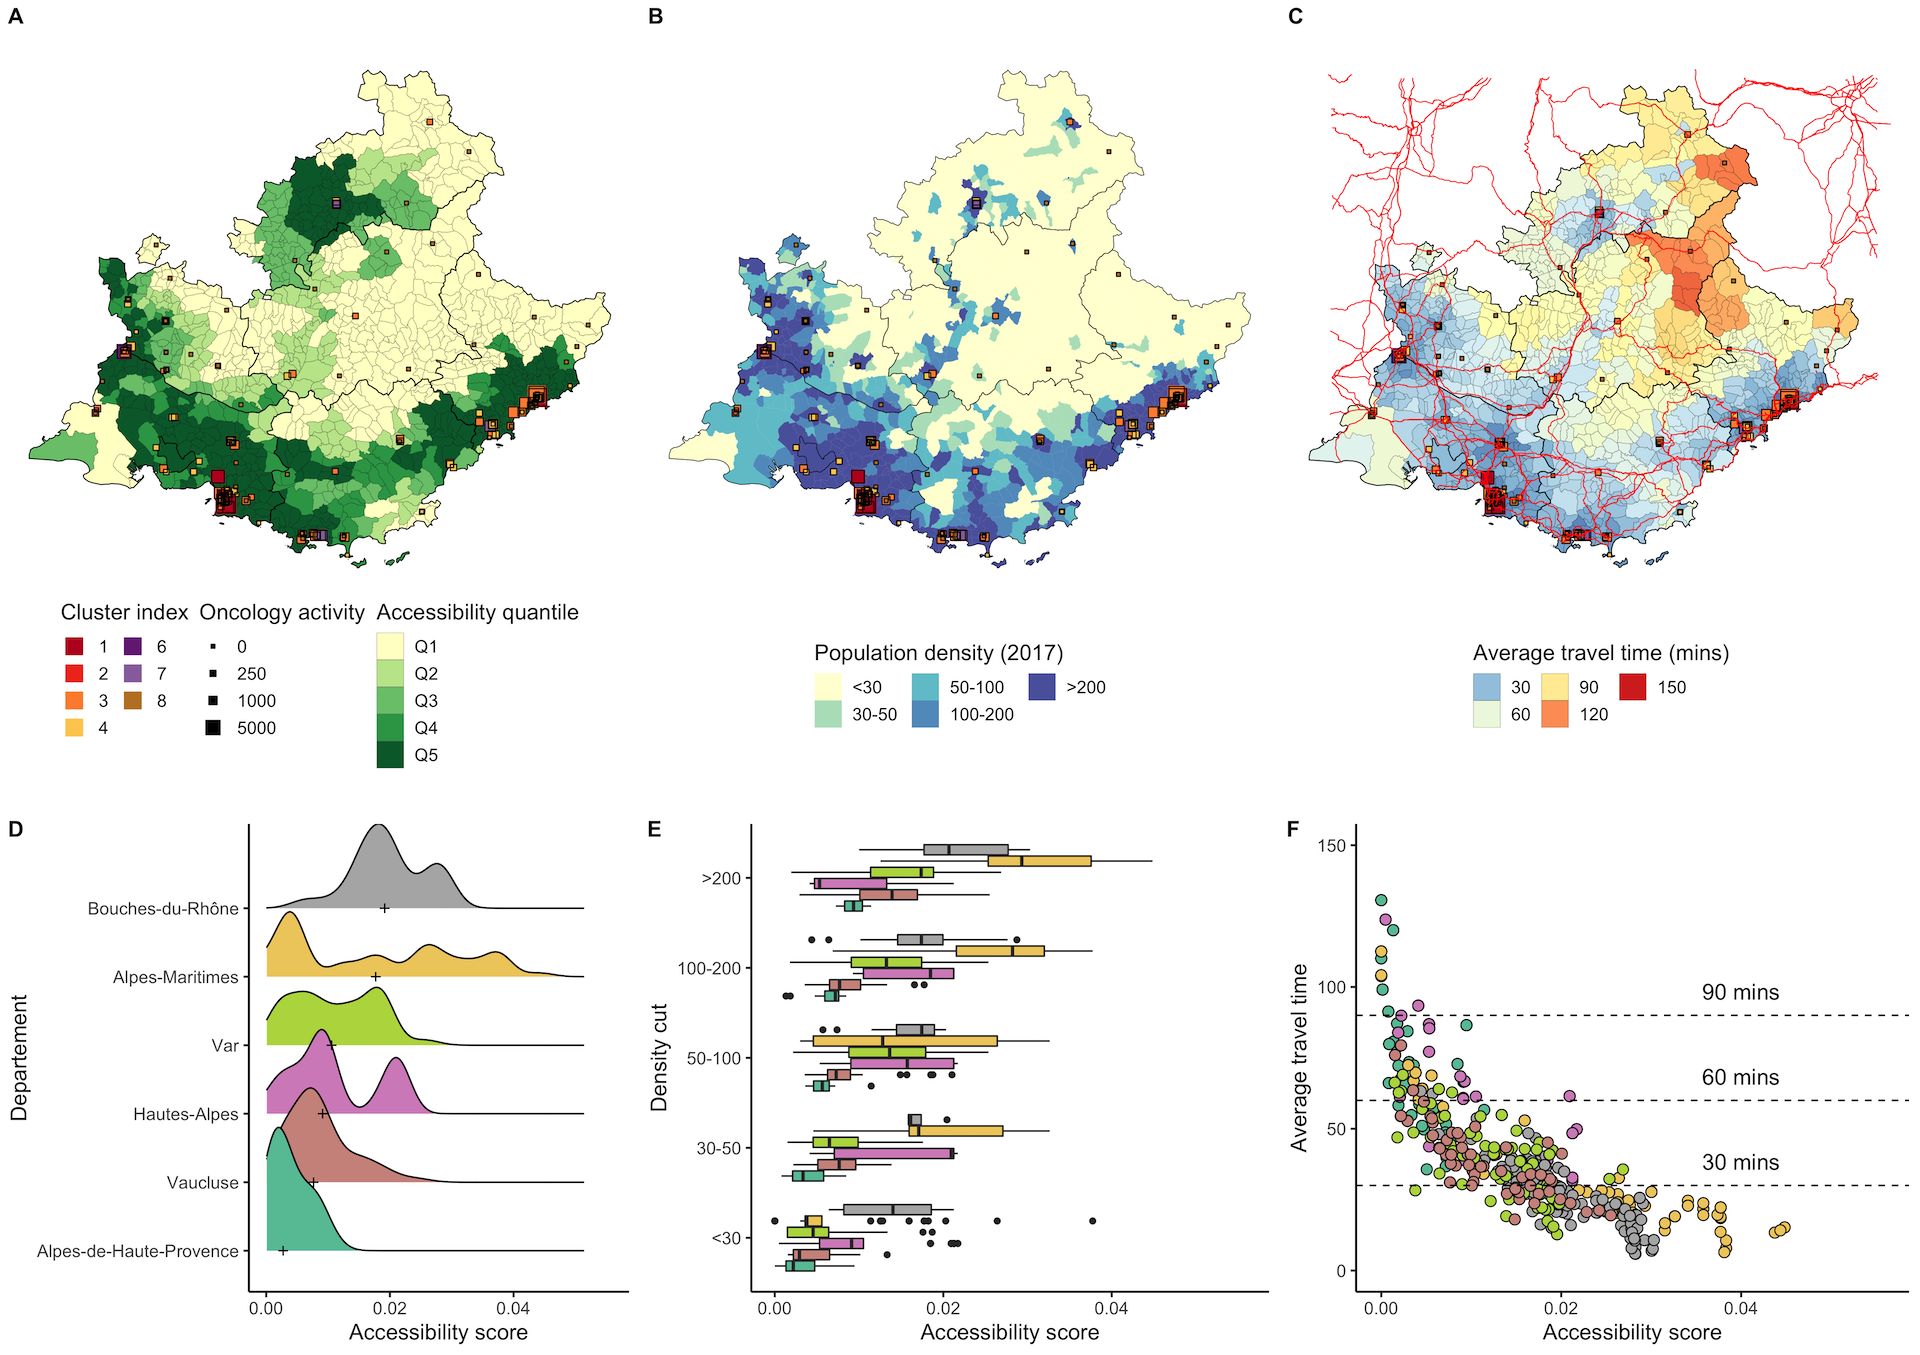
\includegraphics[width=0.9\textwidth]{images/camion/fig4_accessibility_Provence-Alpes-Cote-d'Azur.png}
    \centering
    \caption{
        \textbf{Accessibility distribution in Provence-Alpes-Cote-d'Azur region.} Map (A) shows the region accessibility distribution per municipality. Map (B) displays the population density discretized in 5 bins. The map on plot (C) displays the average travel time for cancer pathways. Large roads (primary, motorway and trucks) are drawn in red. Plot (D) shows the accessibility distribution per department of the region. Plot (E) shows the accessibility distribution by municipality population density and department. Plot (F) compares the accessibility score from municipalities with the average travel time for cancer pathways.
    }
    \label{fig:accessibility-paca}
\end{figure}

\subsection*{Pays de la Loire}

\begin{figure}[H]
    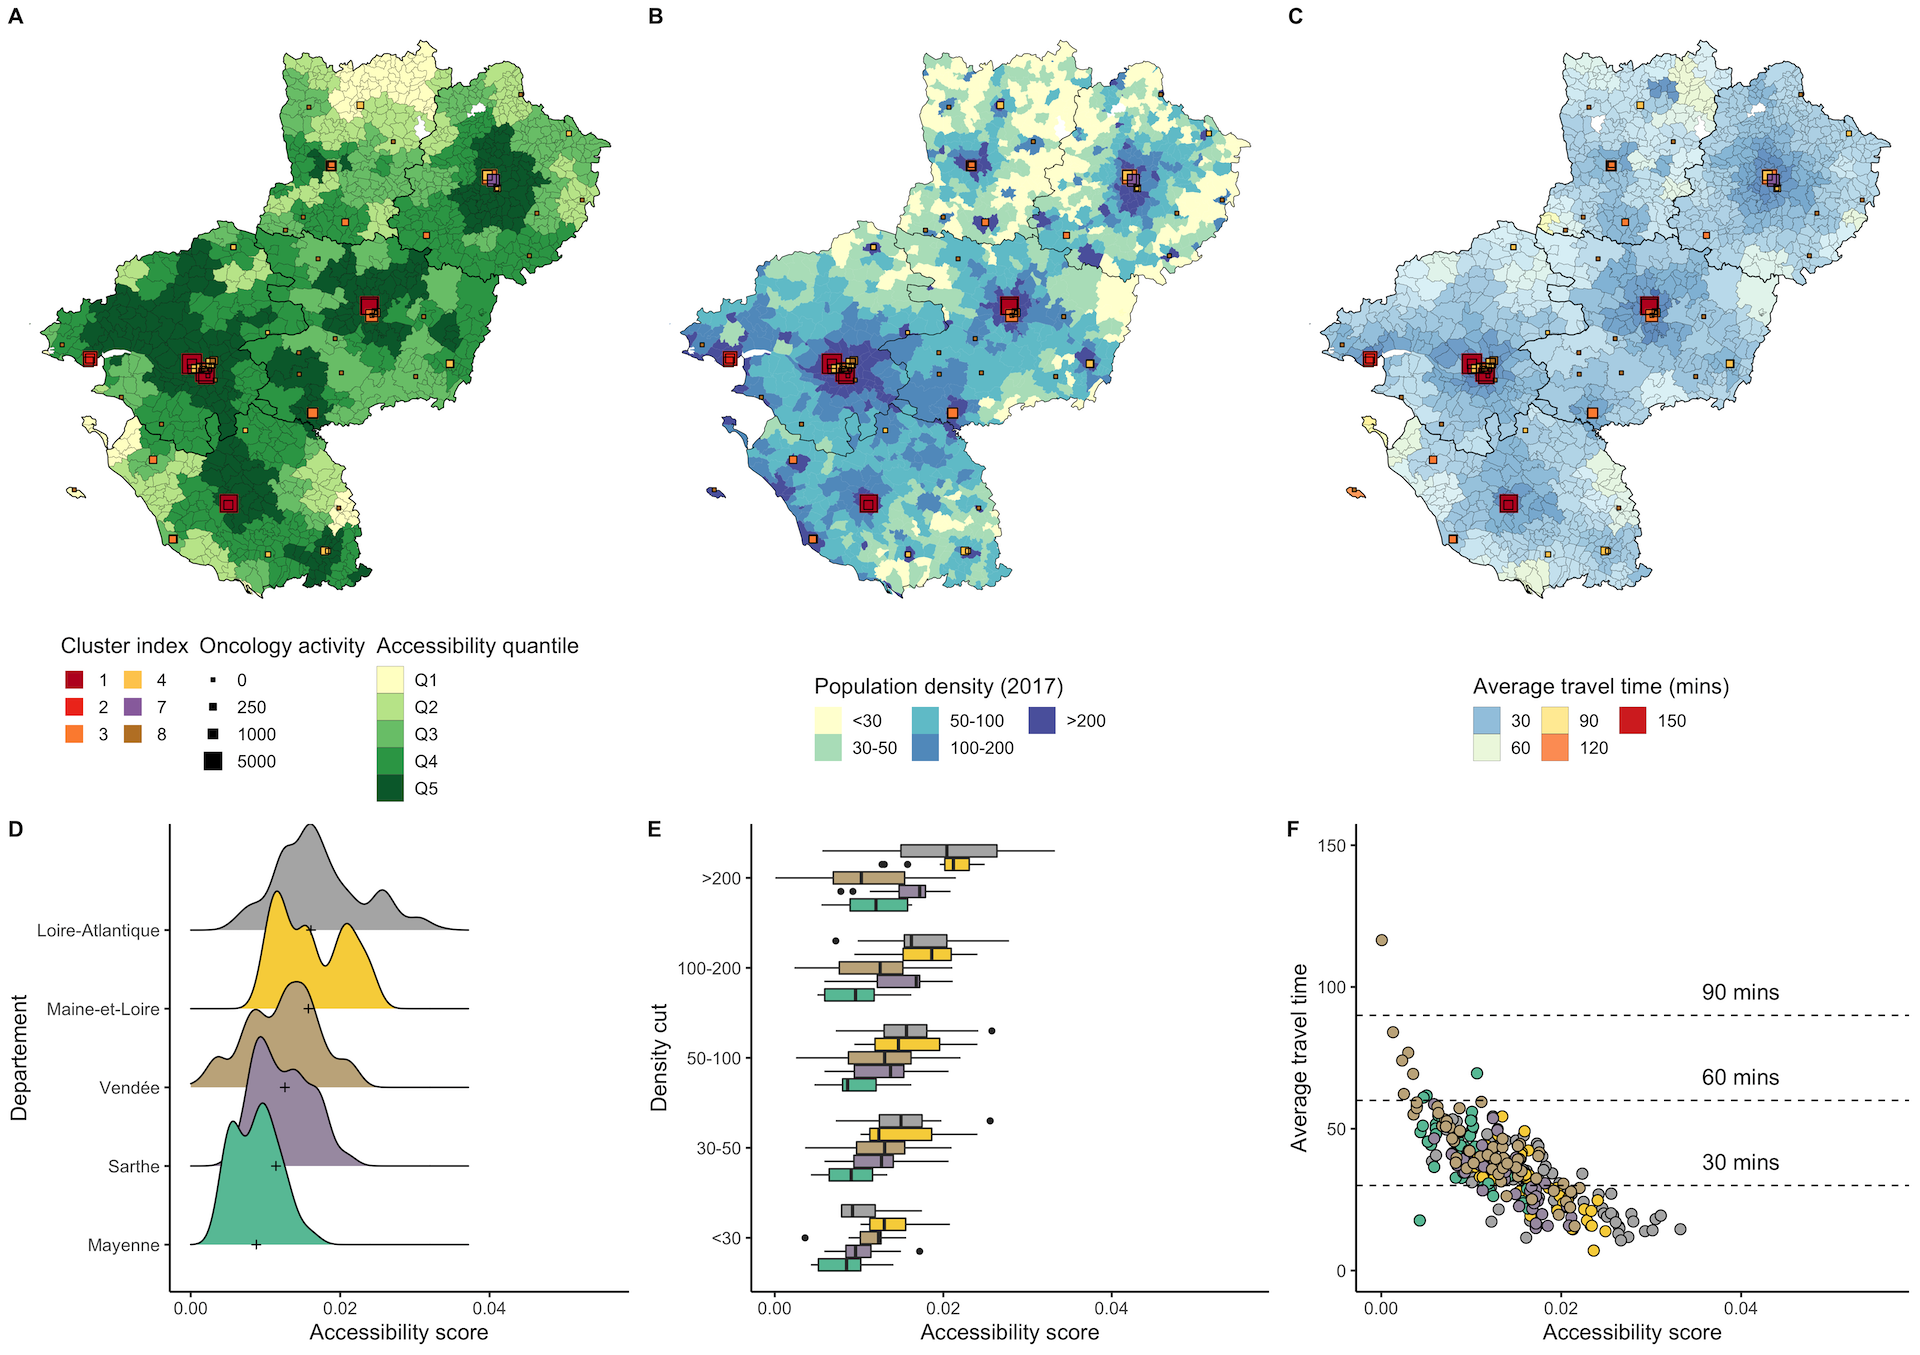
\includegraphics[width=0.9\textwidth]{images/camion/region_accessibility/accessibility_Pays-de-la-Loire.png}
    \centering
    \caption{
        \textbf{Accessibility distribution in Pays-de-la-Loire.}
    }
\end{figure}

\subsection*{Occitanie}

\begin{figure}[H]
    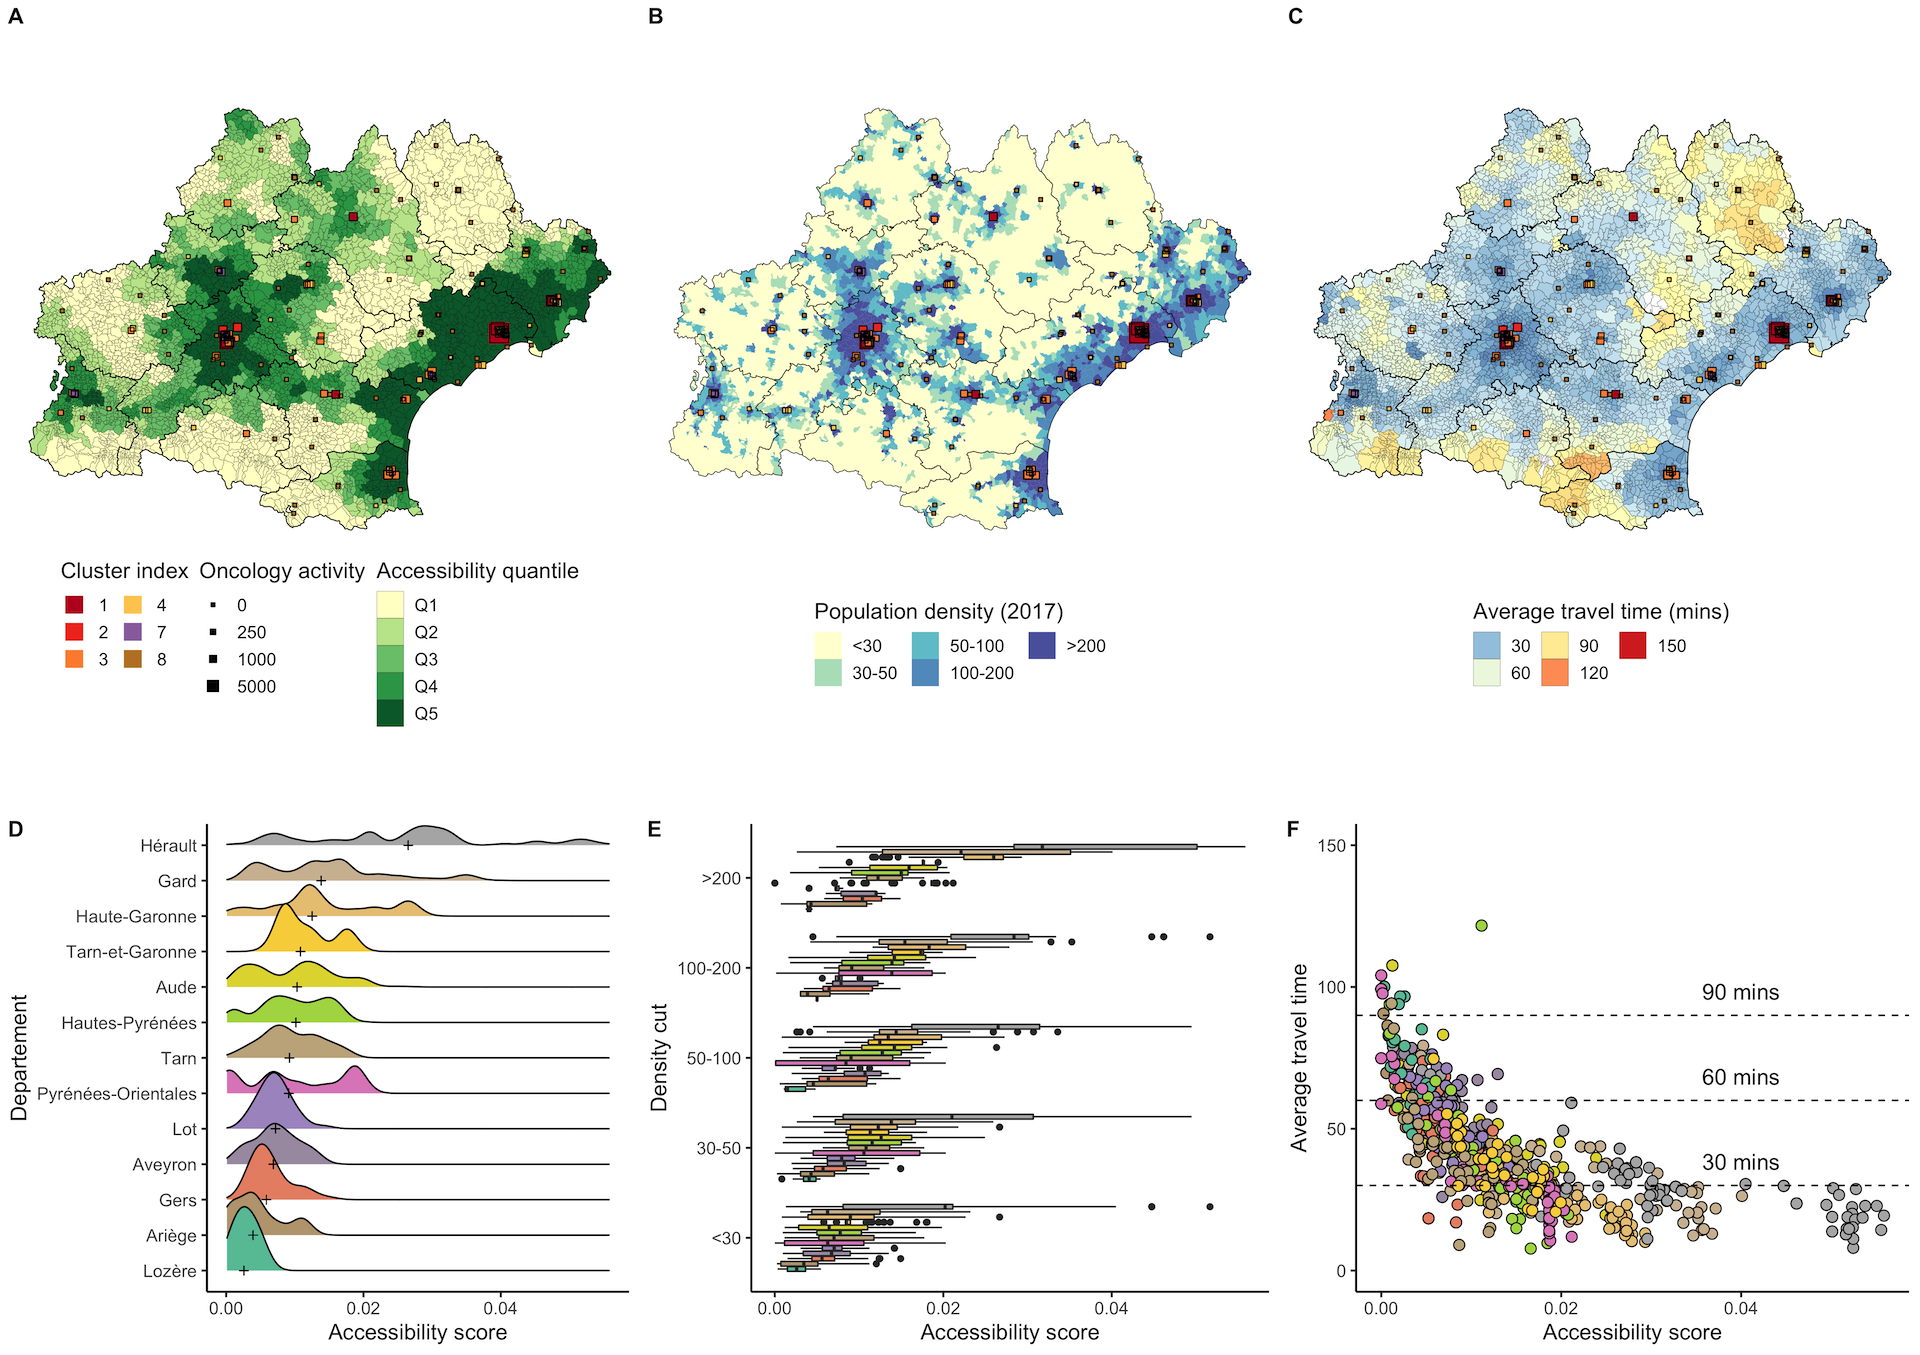
\includegraphics[width=0.9\textwidth]{images/camion/region_accessibility/accessibility_Occitanie.png}
    \centering
    \caption{
        \textbf{Accessibility distribution in Occitanie.}
    }
\end{figure}

\subsection*{Nouvelle-Aquitaine}

\begin{figure}[H]
    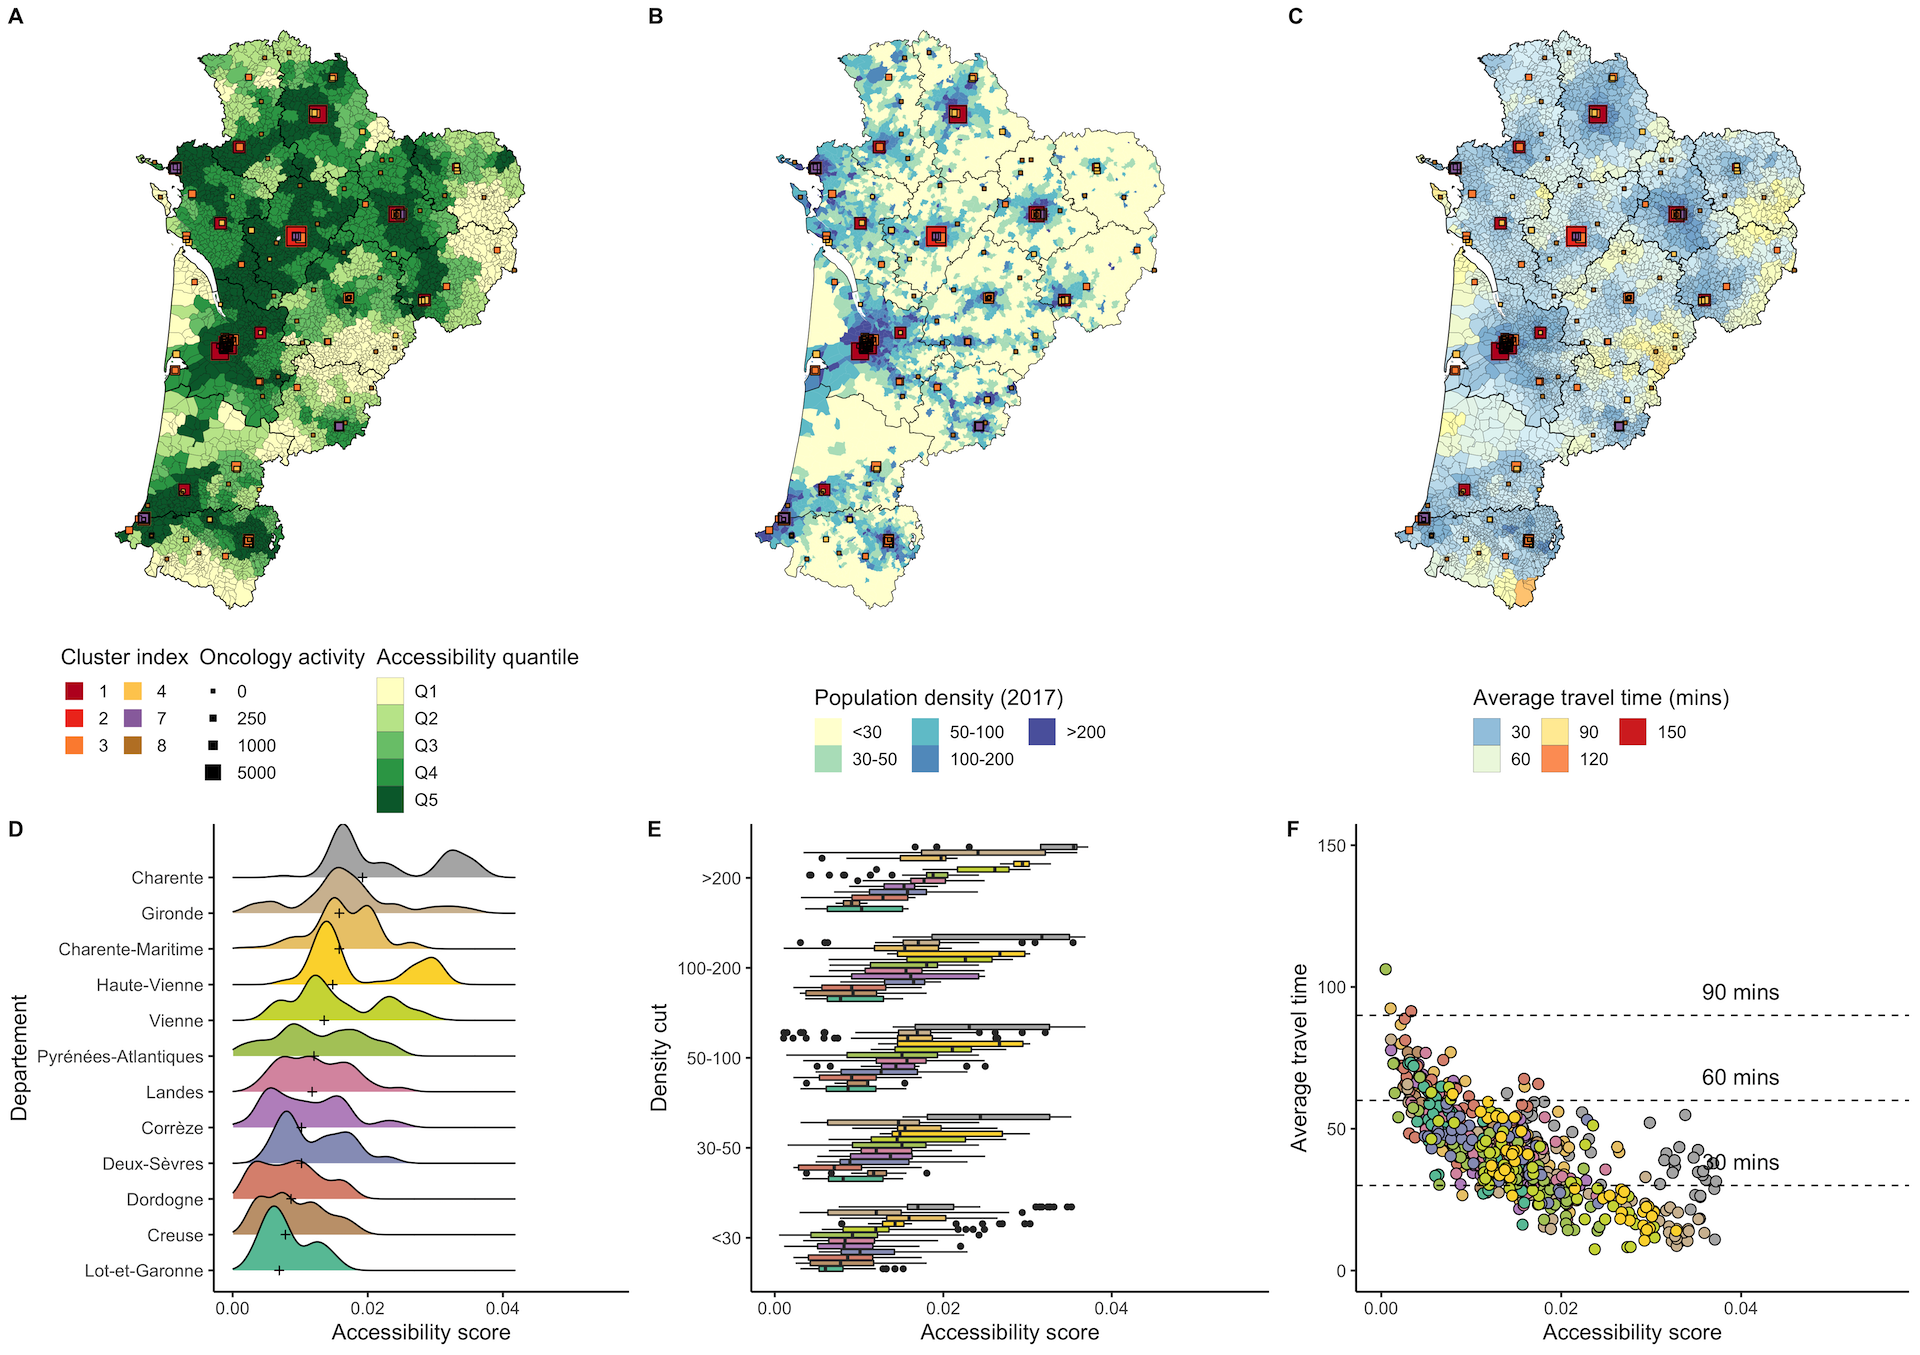
\includegraphics[width=0.9\textwidth]{images/camion/region_accessibility/accessibility_Nouvelle-Aquitaine.png}
    \centering
    \caption{
        \textbf{Accessibility distribution in Nouvelle-Aquitaine.}
    }
\end{figure}

\subsection*{Normandie}

\begin{figure}[H]
    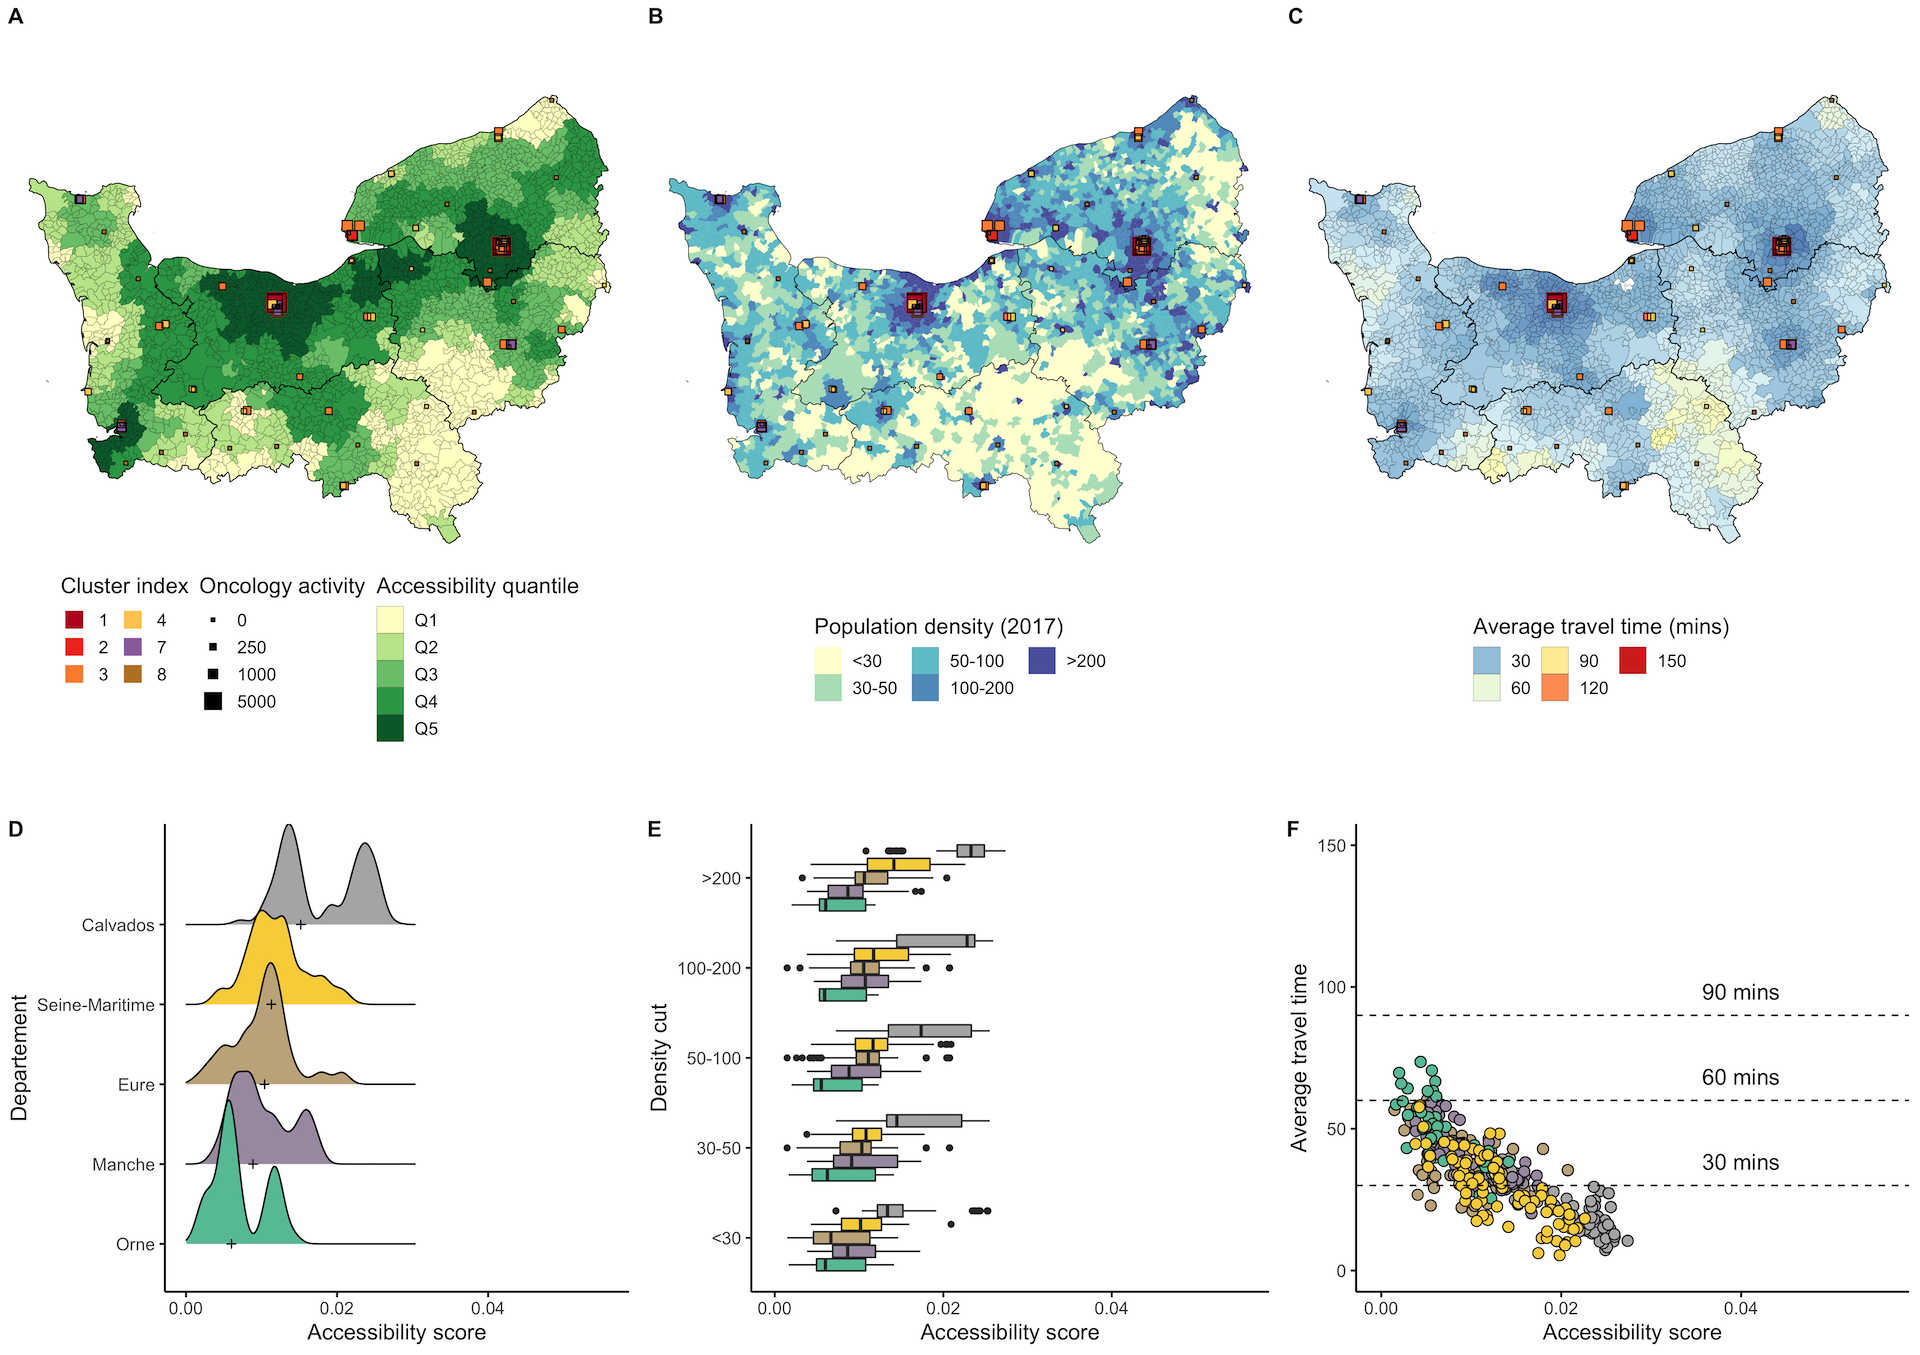
\includegraphics[width=0.9\textwidth]{images/camion/region_accessibility/accessibility_Normandie.png}
    \centering
    \caption{
        \textbf{Accessibility distribution in Normandie.}
    }
\end{figure}

\subsection*{Île-de-France}

\begin{figure}[H]
    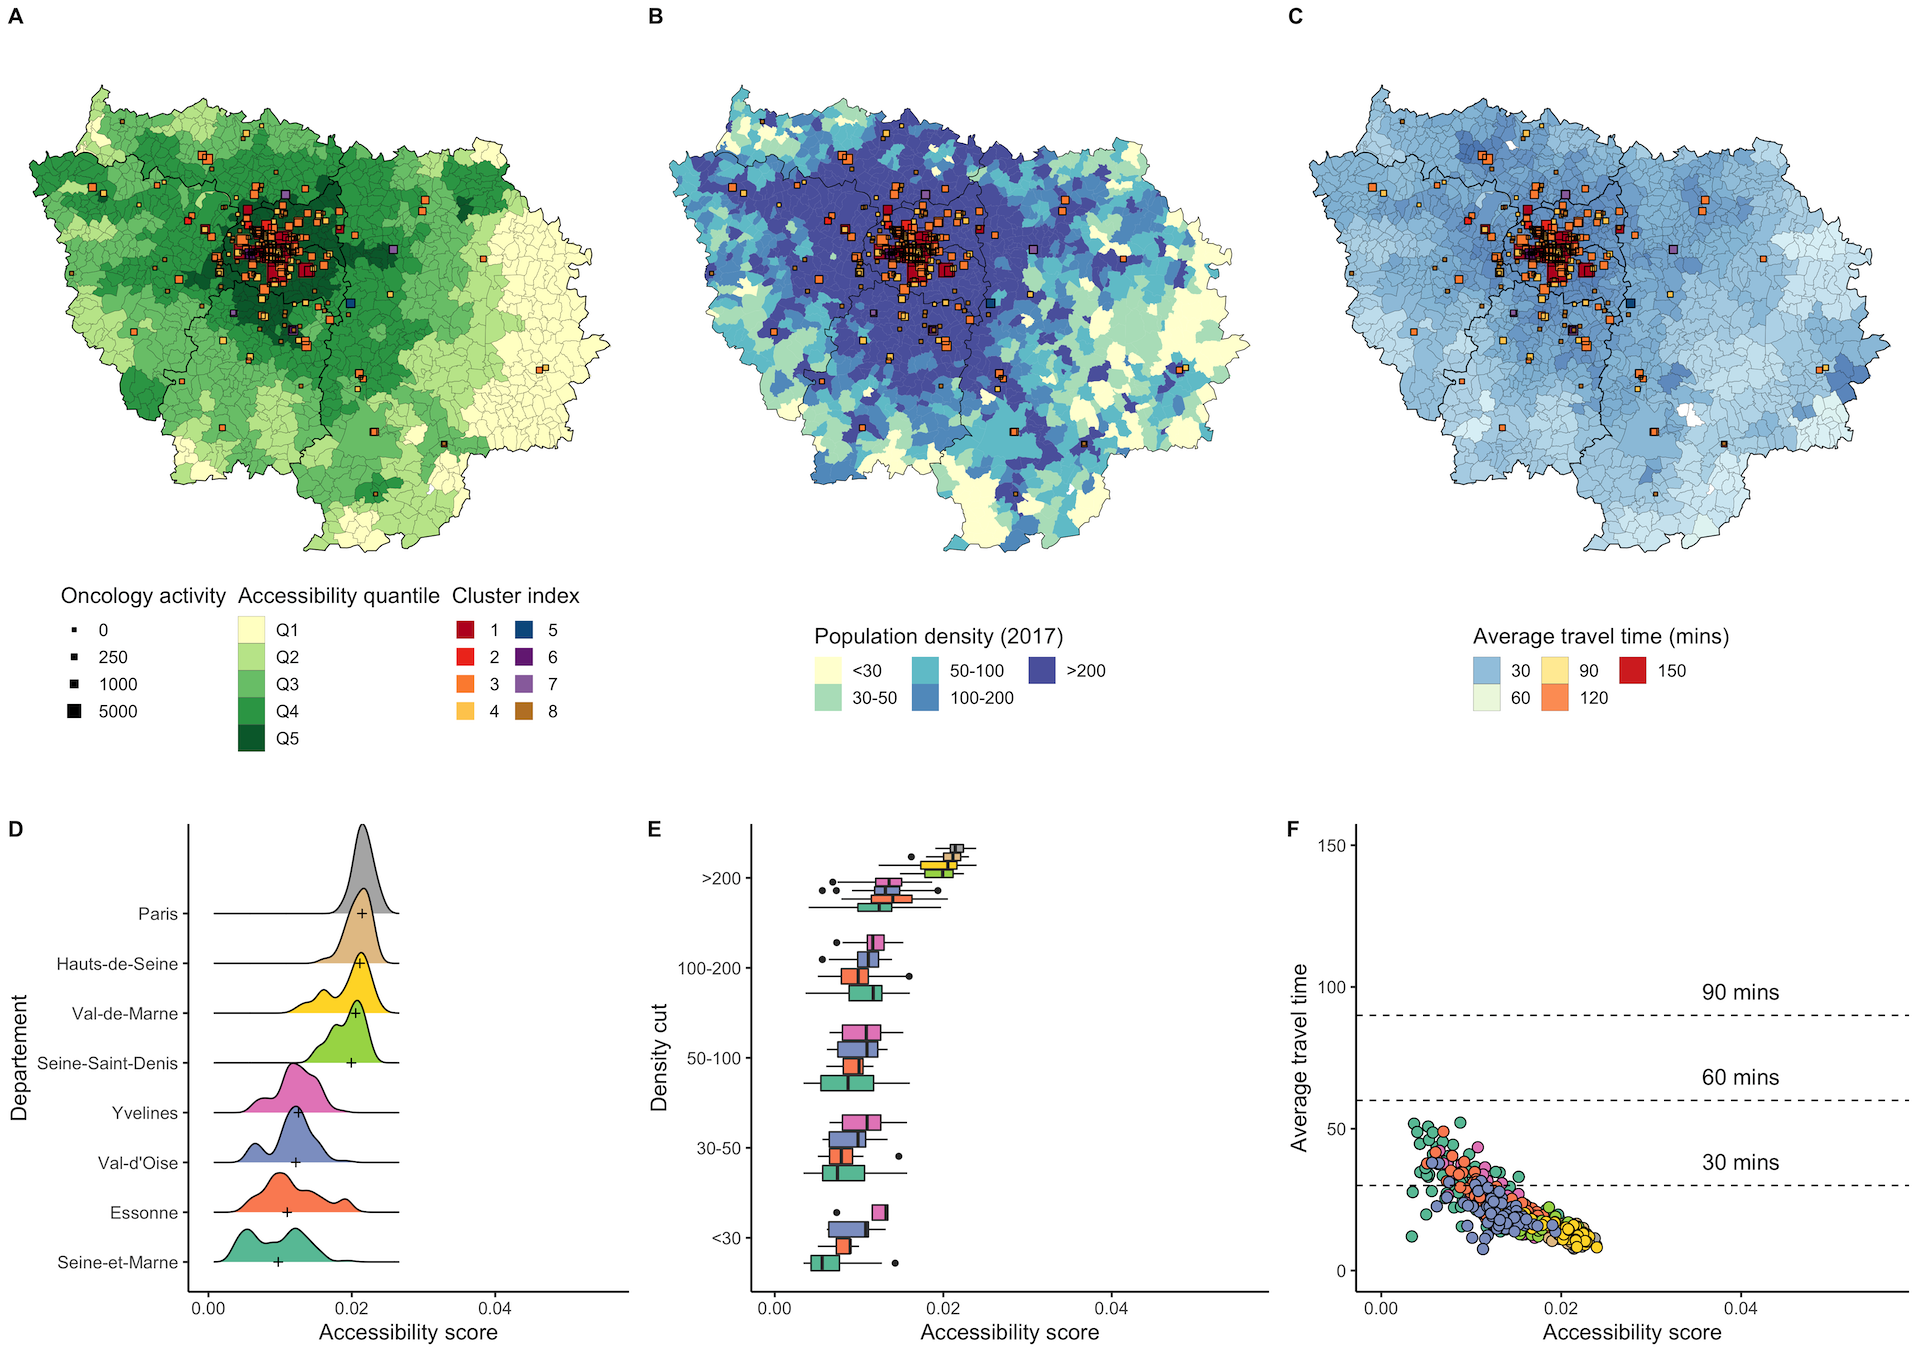
\includegraphics[width=0.9\textwidth]{images/camion/region_accessibility/accessibility_Ile-de-France.png}
    \centering
    \caption{
        \textbf{Accessibility distribution in Ile-de-France.}
    }
\end{figure}

\subsection*{Hauts-de-France}

\begin{figure}[H]
    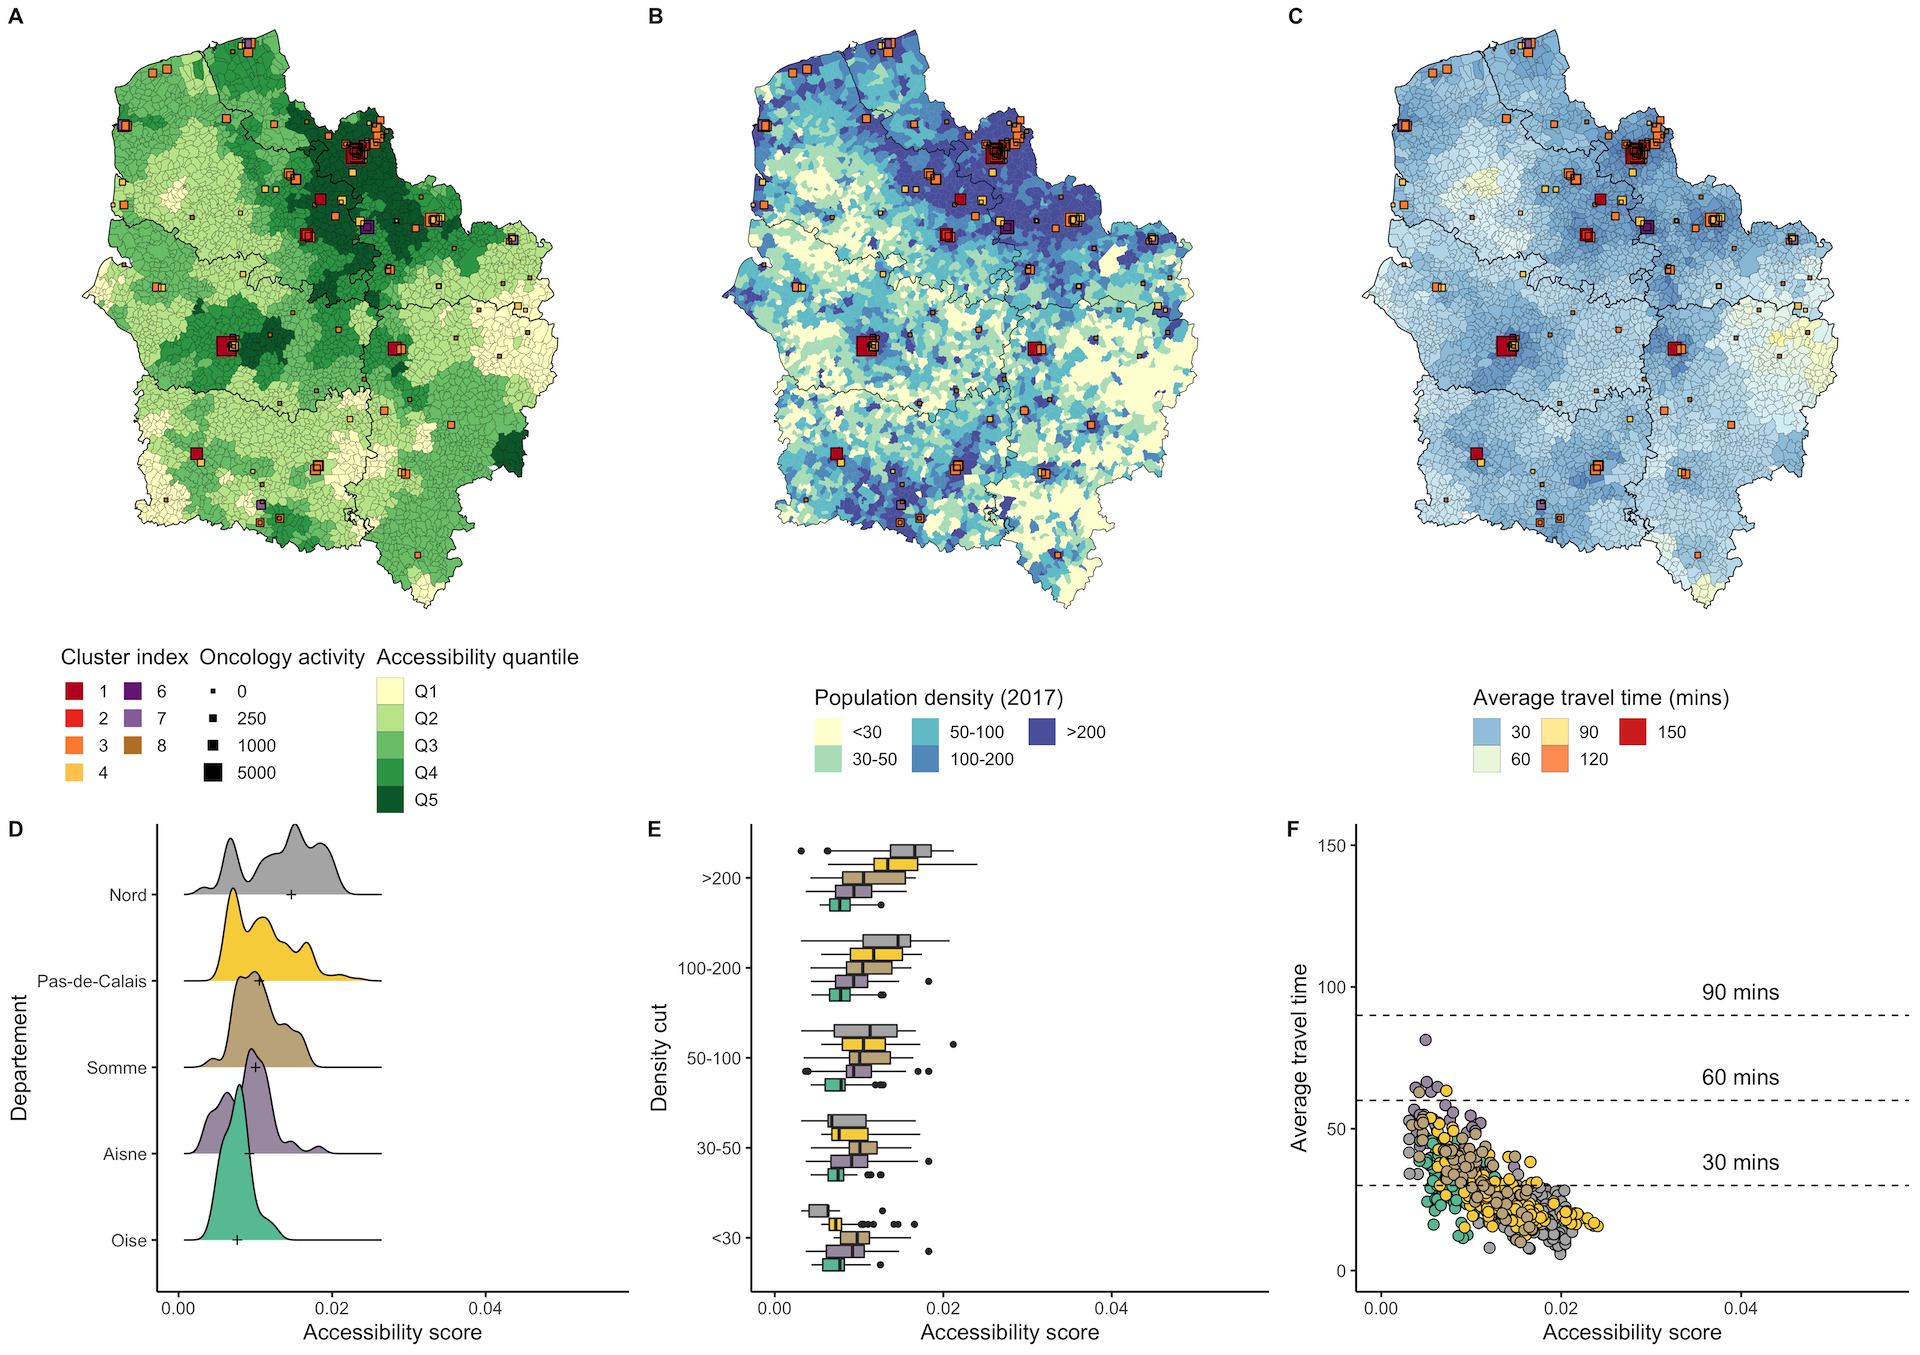
\includegraphics[width=0.9\textwidth]{images/camion/region_accessibility/accessibility_Hauts-de-France.png}
    \centering
    \caption{
        \textbf{Accessibility distribution in Hauts-de-France.}
    }
\end{figure}

\subsection*{Grand Est}

\begin{figure}[H]
    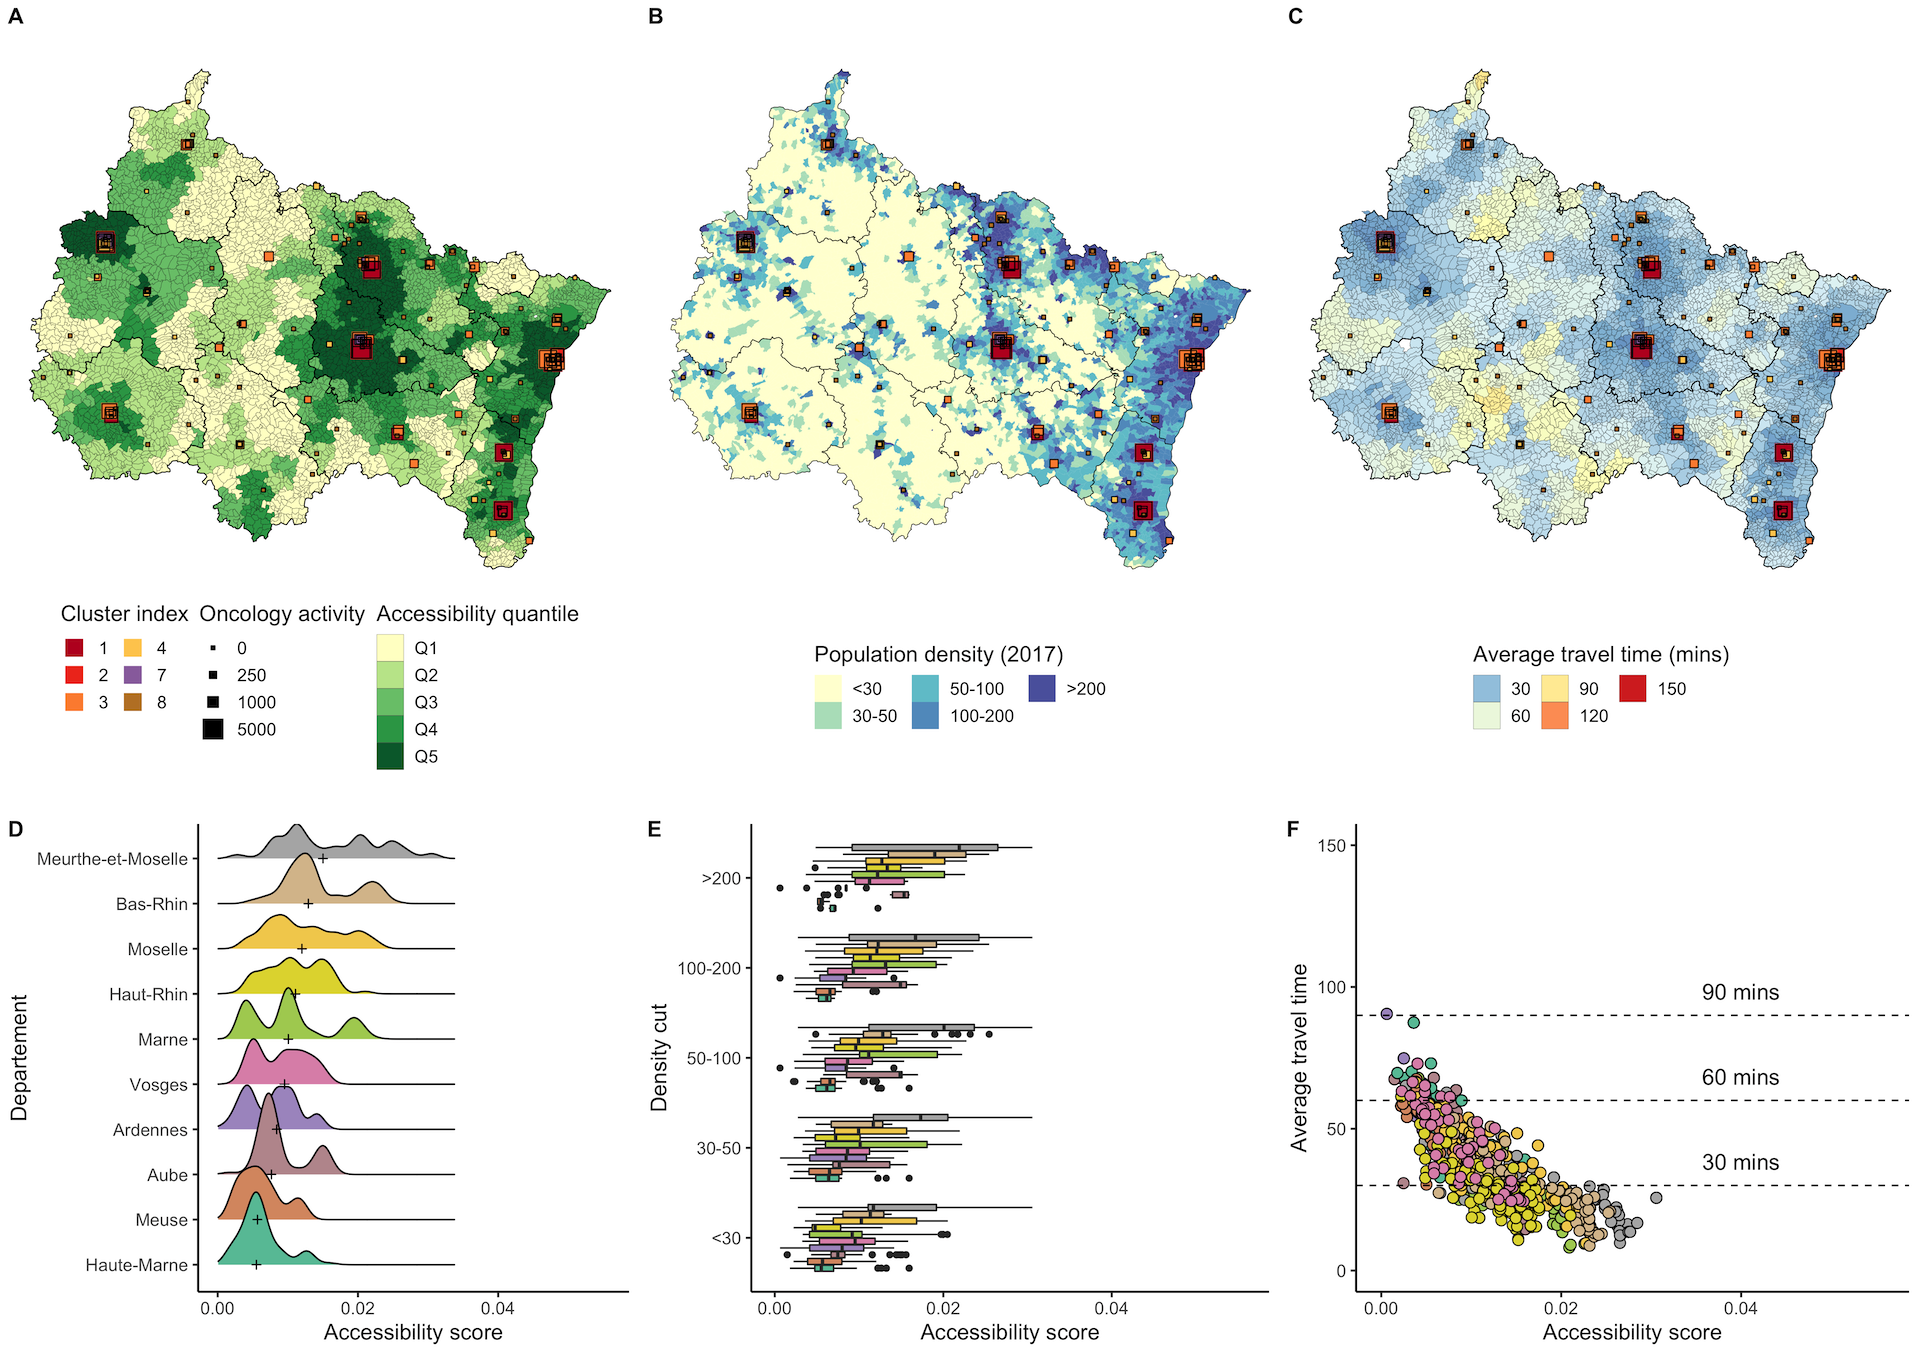
\includegraphics[width=0.9\textwidth]{images/camion/region_accessibility/accessibility_Grand-Est.png}
    \centering
    \caption{
        \textbf{Accessibility distribution in Grand-Est.}
    }
\end{figure}

\subsection*{Centre-Val de Loire}

\begin{figure}[H]
    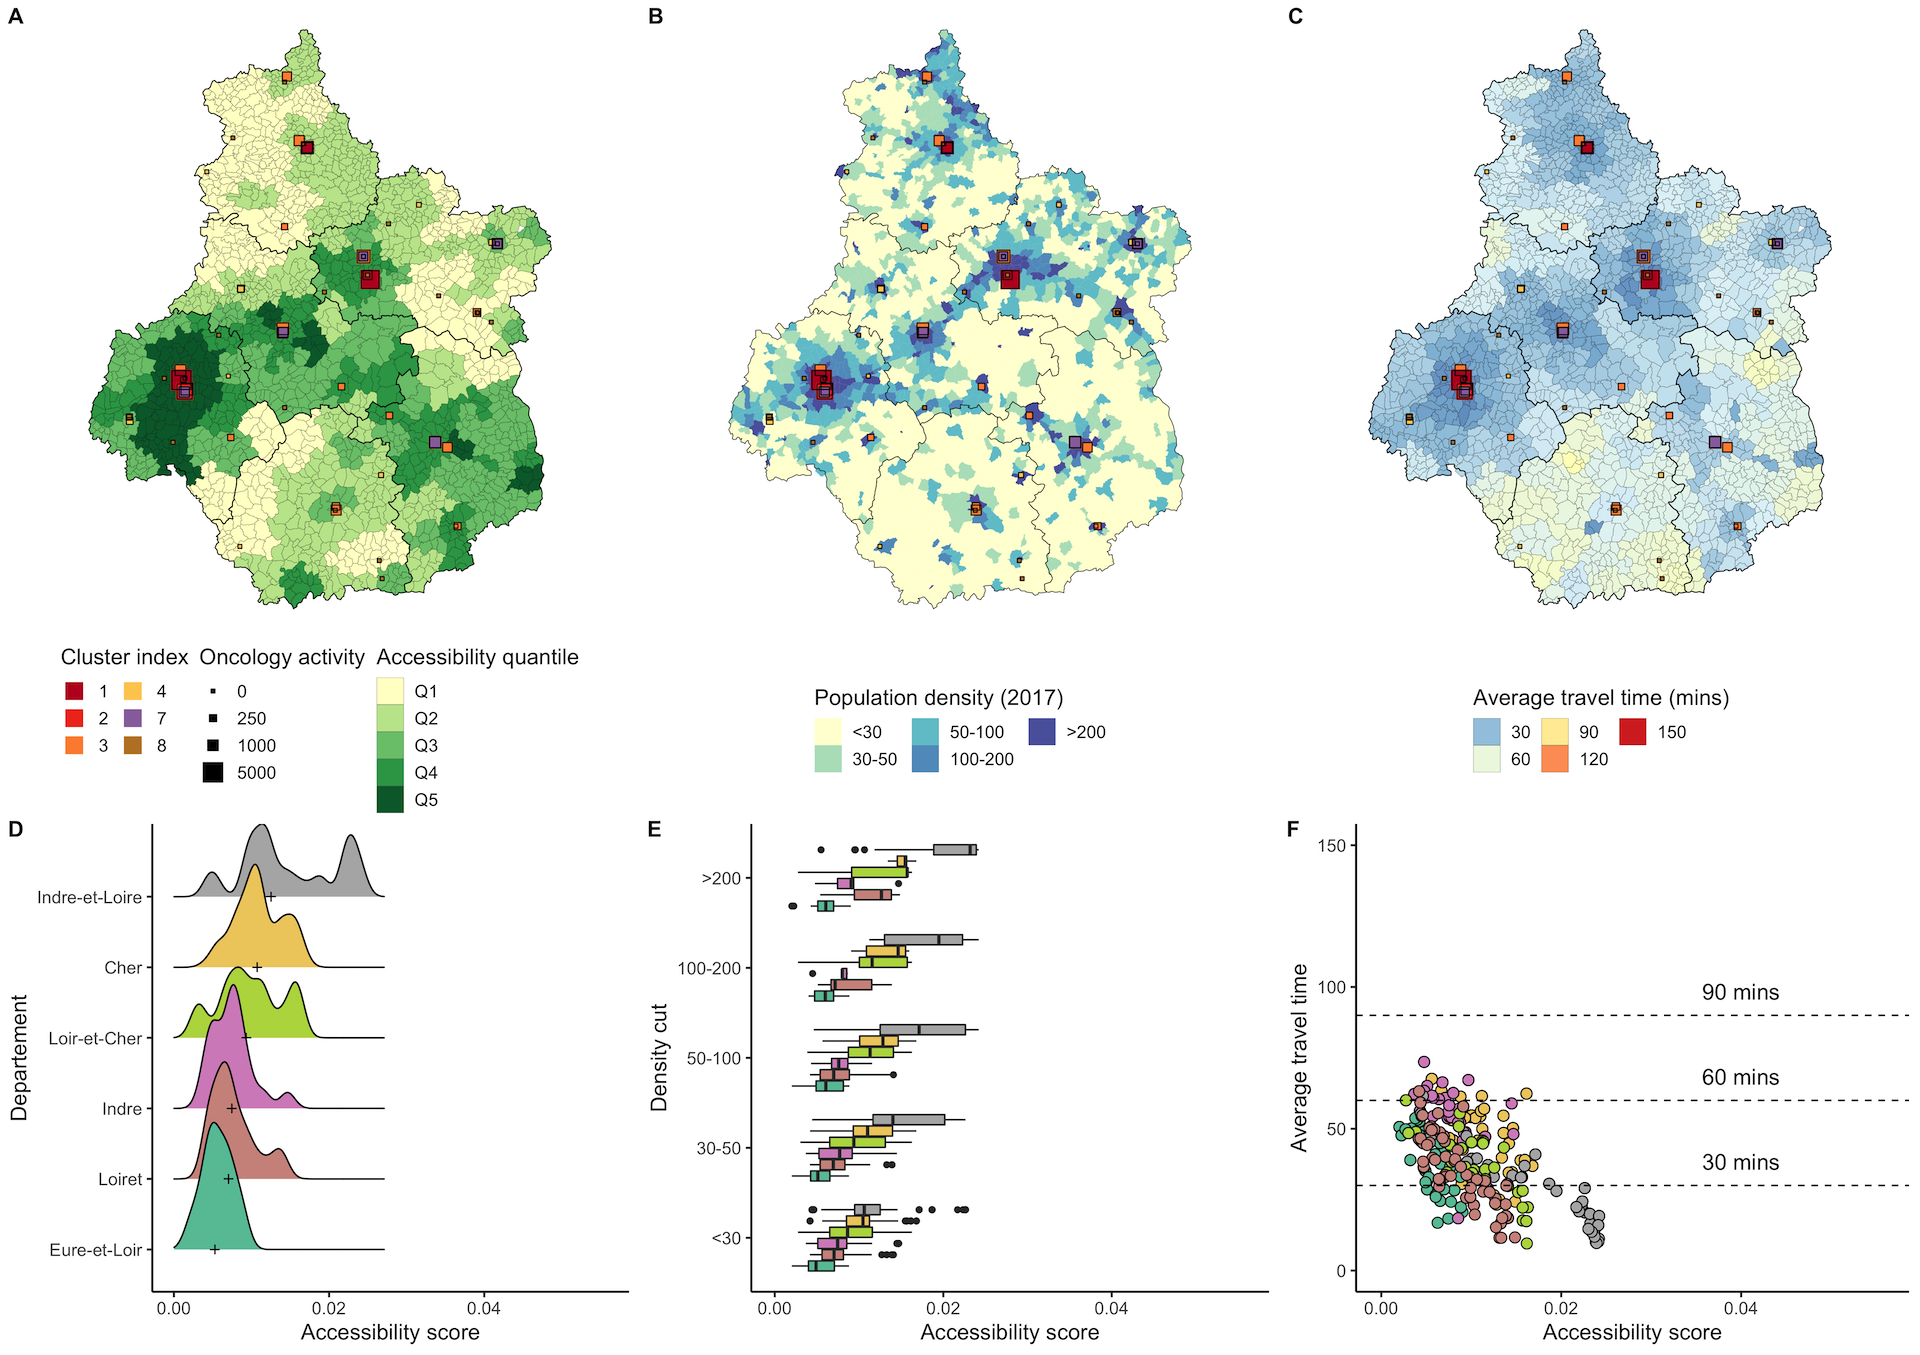
\includegraphics[width=0.9\textwidth]{images/camion/region_accessibility/accessibility_Centre-Val-de-Loire.png}
    \centering
    \caption{
        \textbf{Accessibility distribution in Centre Val de Loire.}
    }
\end{figure}

\subsection*{Bretagne}

\begin{figure}[H]
    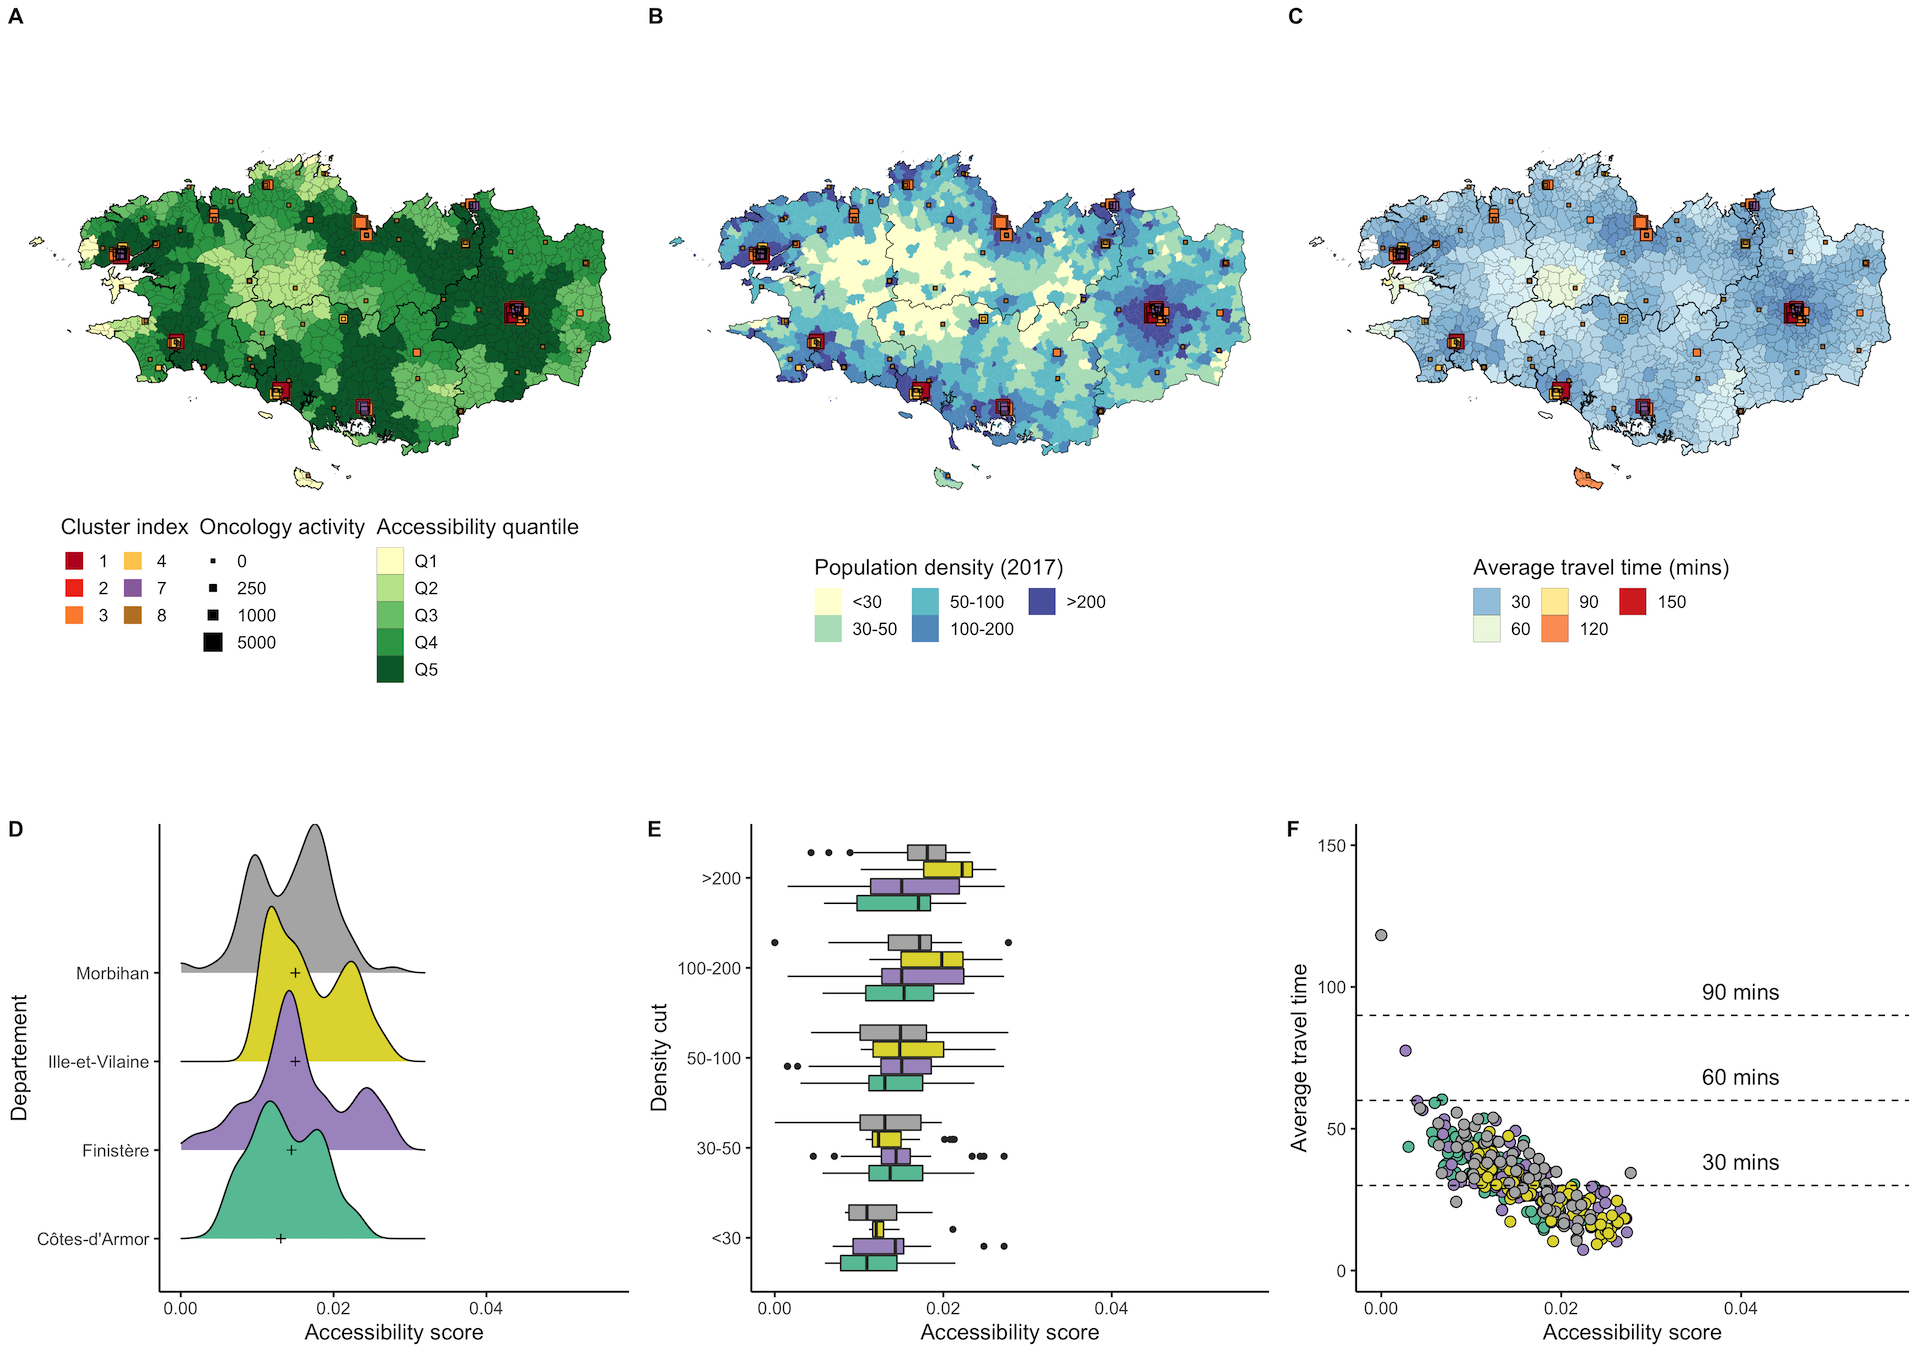
\includegraphics[width=0.9\textwidth]{images/camion/region_accessibility/accessibility_Bretagne.png}
    \centering
    \caption{
        \textbf{Accessibility distribution in Bretagne.}
    }
\end{figure}

\subsection*{Bourgogne-Franche-Comté}

\begin{figure}[H]
    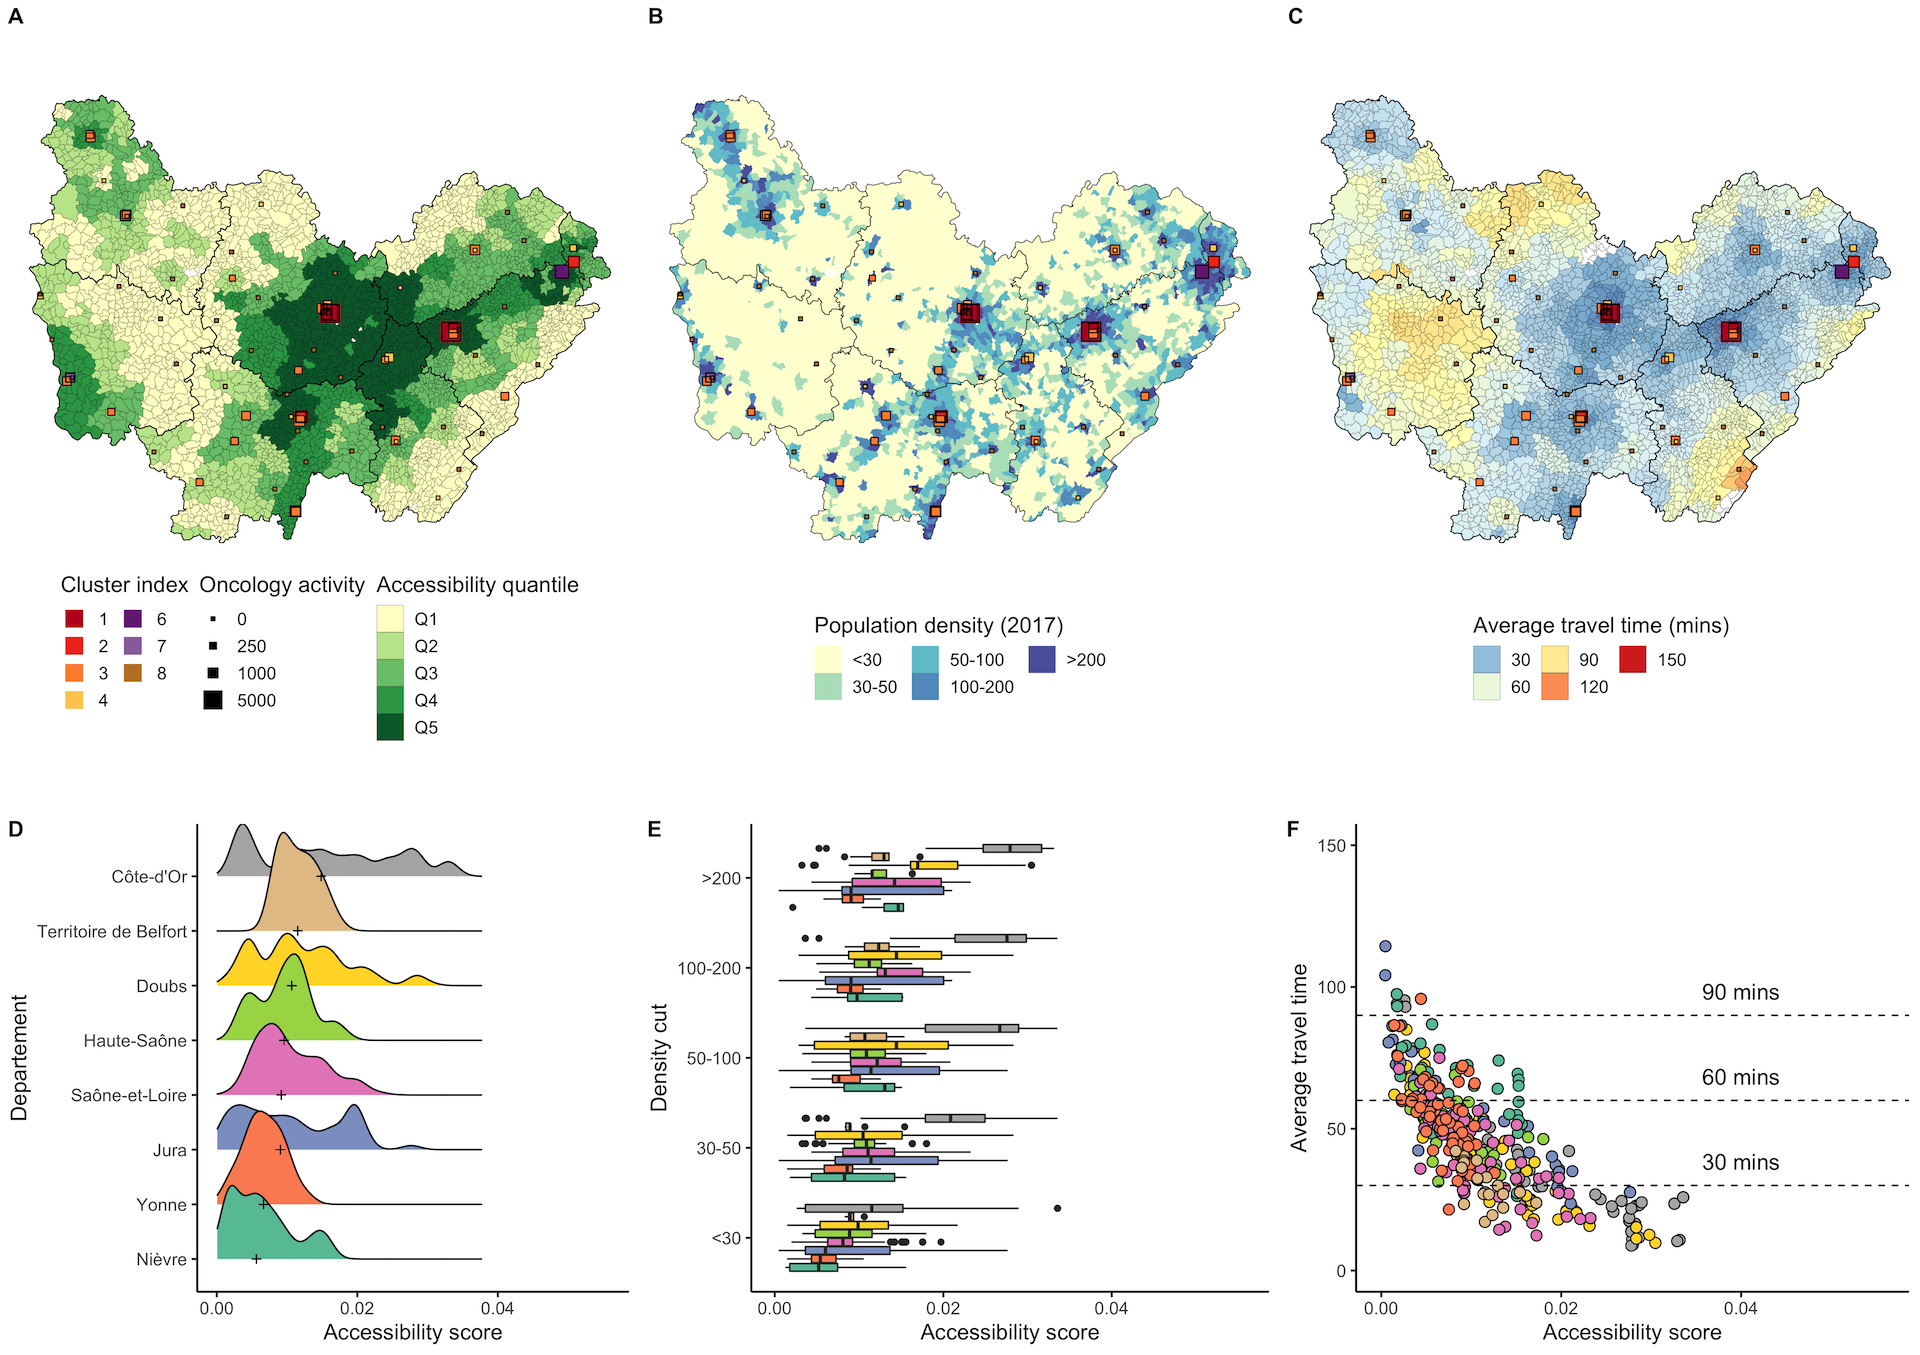
\includegraphics[width=0.9\textwidth]{images/camion/region_accessibility/accessibility_Bourgogne-Franche-Comte.png}
    \centering
    \caption{
        \textbf{Accessibility distribution in Bourgogne-Franche-Comté.}
    }
\end{figure}

\subsection*{Auvergne-Rhône-Alpes}

\begin{figure}[H]
    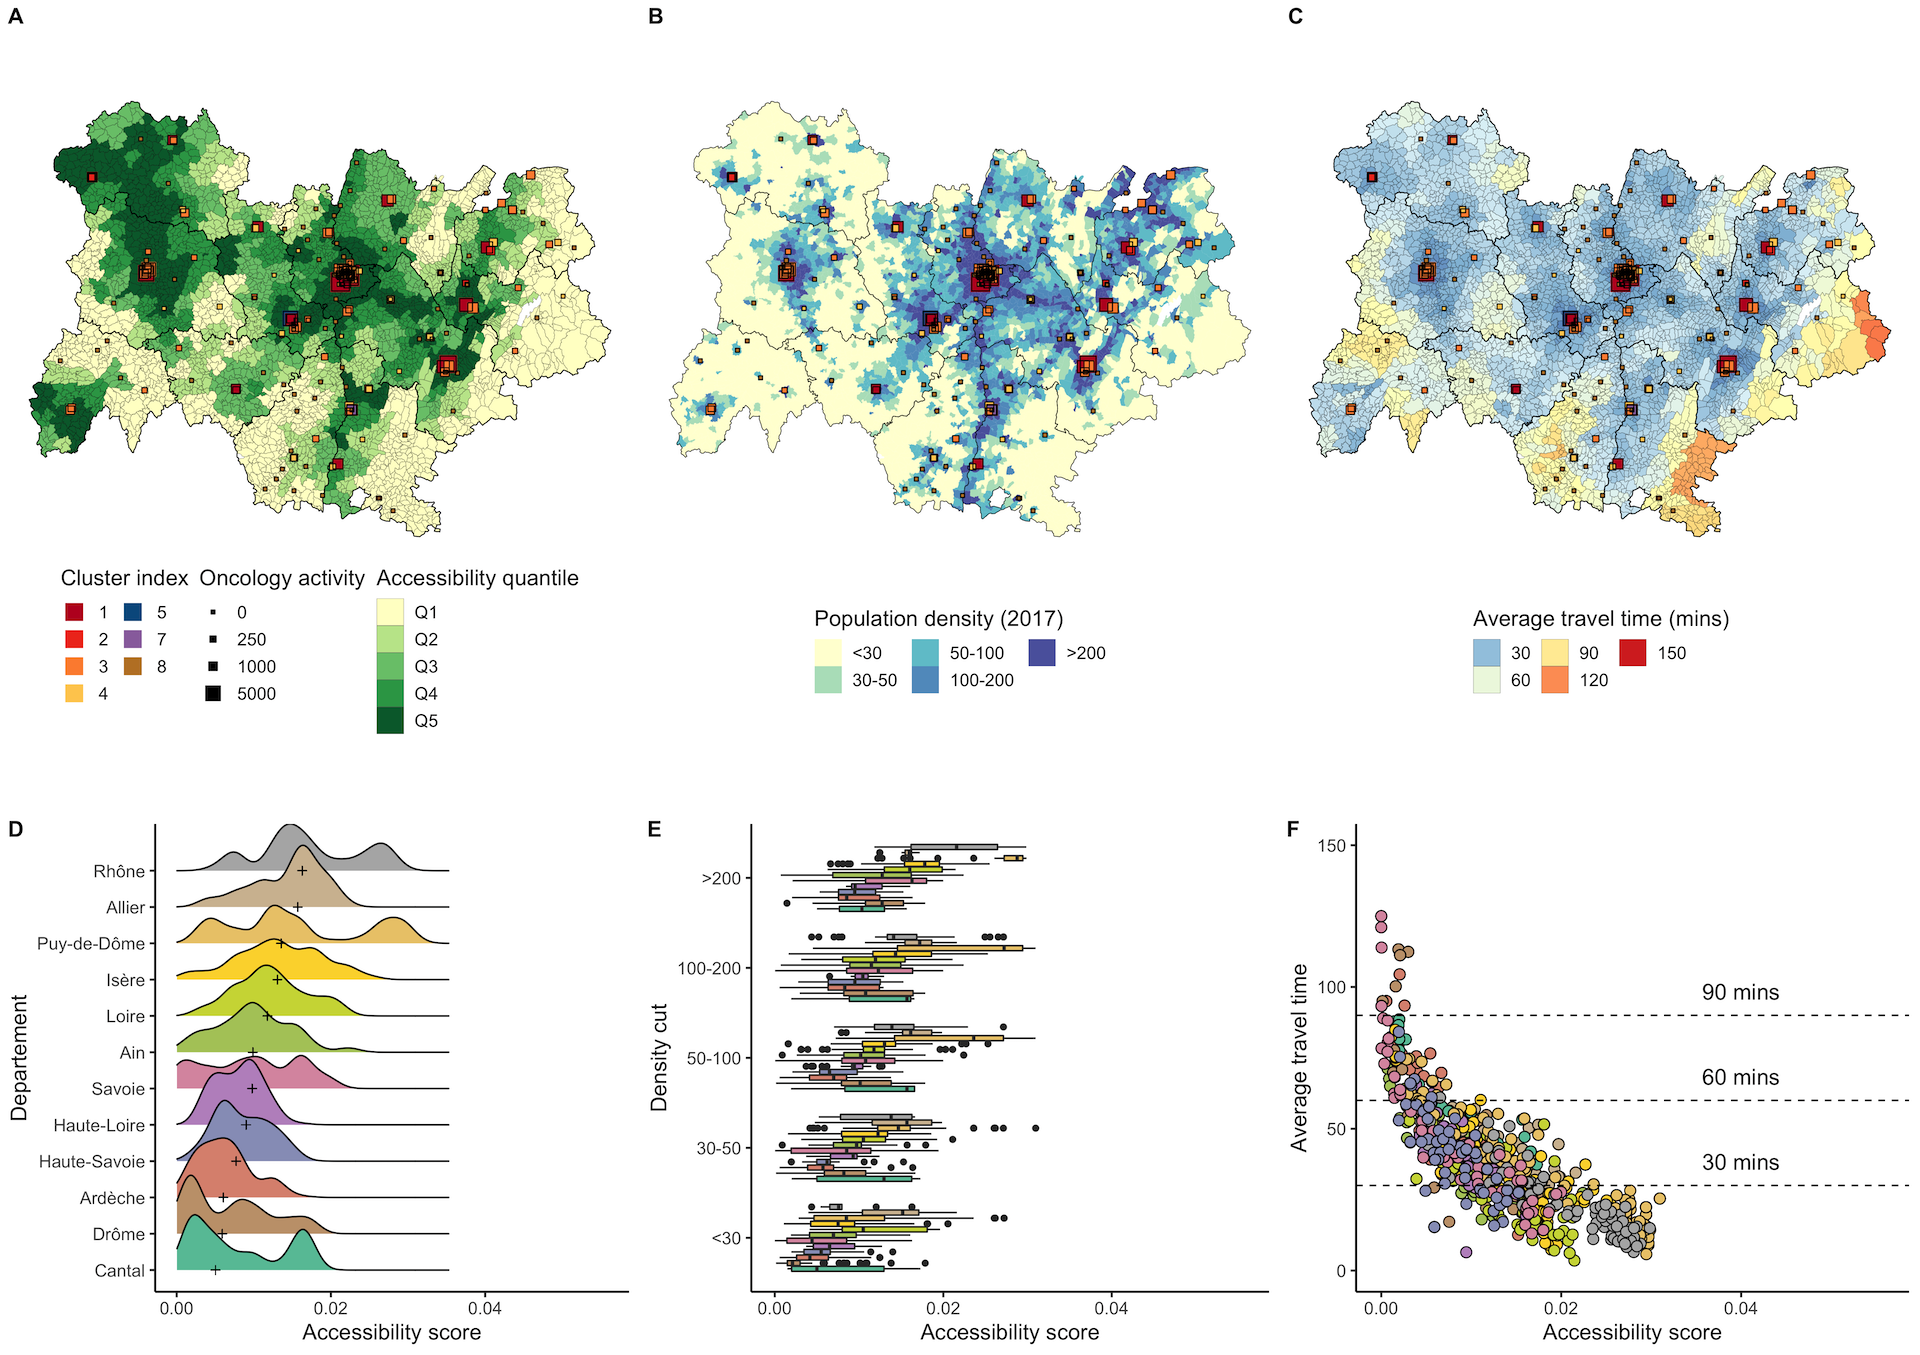
\includegraphics[width=0.9\textwidth]{images/camion/region_accessibility/accessibility_Auvergne-Rhone-Alpes.png}
    \centering
    \caption{
        \textbf{Accessibility distribution in Auvergne-Rhone-Alpes.}
    }
\end{figure}

\section{Discussion}

Specific attention should be given to municipalities with very poor access to oncology care centers. While we saw that most of the population lives in high accessibility areas, around 6\% of the population lives in the bottom 20\% accessibility quantile. Among these municipalities, some are very rural and mountainous like those in the Alpes-de-Haute-Provence in Provence-Alpes-Cote-d'Azur region. Such areas cannot be expected to have a very good healthcare coverage. By contrast, the case of suburban areas with relatively dense population and poor accessibility should be addressed more easily. Our optimization algorithm can help driving public health policies, as it effectively identifies areas where accessibility could grow, by allocating additional oncology activity to a restricted number of care centers. The proposed growth factors are indicative and do not have to be effective within a year, as it represents a considerable effort for care centers to increase their activity.
Our oncology accessibility score is deliberately non-specific to cancer type. This score is meant to outline how easy it would be for a population location to reach a first entry point for oncology care. Here, we are only focusing on surgery, chemotherapy, and radiotherapy treatments. The same technique could be used on a specific cancer type, the method will remain the same, only the supply variable used in the accessibility score will change. We should mention that \ac{sa} is better suited for pathologies that are relatively well handled across the whole country. Accessibility for rare diseases like pediatric cancer or complex cancers that re-quire a specific expertise is less informative because only a handful of care centers are indicated.
Similarly, we could compute an accessibility score that is focused on specific kinds of stays: our web application lets the user pick between surgery, chemotherapy, or radiotherapy as supply variable.

\section{Oncology Accessibility web application}

% TODO
